%%%%%%%%%%%%%%%%%%%%%%%%%%%%%%%%%%%%%%%%%
% Short Sectioned Assignment LaTeX Template Version 1.0 (5/5/12)
% This template has been downloaded from: http://www.LaTeXTemplates.com
% Original author:  Frits Wenneker (http://www.howtotex.com)
% License: CC BY-NC-SA 3.0 (http://creativecommons.org/licenses/by-nc-sa/3.0/)
%%%%%%%%%%%%%%%%%%%%%%%%%%%%%%%%%%%%%%%%%

% \documentclass[paper=a4, fontsize=11pt]{scrartcl} % A4 paper and 11pt font size
\documentclass[11pt, a4paper]{book}
\usepackage[T1]{fontenc} % Use 8-bit encoding that has 256 glyphs
\usepackage[utf8]{inputenc}
\usepackage{fourier} % Use the Adobe Utopia font for the document - comment this line to return to the LaTeX default
\usepackage{listings} % para insertar código con formato similar al editor
\usepackage[spanish, es-tabla]{babel} % Selecciona el español para palabras introducidas automáticamente, p.ej. "septiembre" en la fecha y especifica que se use la palabra Tabla en vez de Cuadro
\usepackage{url} % ,href} %para incluir URLs e hipervínculos dentro del texto (aunque hay que instalar href)
\usepackage{graphics,graphicx, float} %para incluir imágenes y colocarlas
\usepackage[gen]{eurosym} %para incluir el símbolo del euro
\usepackage{cite} %para incluir citas del archivo <nombre>.bib
\usepackage{enumerate}
\usepackage{hyperref}
\usepackage{graphicx}
\usepackage{tabularx}
\usepackage{booktabs}

\usepackage[table,xcdraw]{xcolor}
\hypersetup{
	colorlinks=true,	% false: boxed links; true: colored links
	linkcolor=black,	% color of internal links
	urlcolor=cyan		% color of external links
}
\renewcommand{\familydefault}{\sfdefault}
\usepackage{fancyhdr} % Custom headers and footers
\pagestyle{fancyplain} % Makes all pages in the document conform to the custom headers and footers
\fancyhead[L]{} % Empty left header
\fancyhead[C]{} % Empty center header
\fancyhead[R]{Pablo Millán Cubero} % My name
\fancyfoot[L]{} % Empty left footer
\fancyfoot[C]{} % Empty center footer
\fancyfoot[R]{\thepage} % Page numbering for right footer
%\renewcommand{\headrulewidth}{0pt} % Remove header underlines
\renewcommand{\footrulewidth}{0pt} % Remove footer underlines
\setlength{\headheight}{13.6pt} % Customize the height of the header
\setlength{\parskip}{0.5em}

\usepackage{titlesec, blindtext, color}
\definecolor{gray75}{gray}{0.75}
\newcommand{\hsp}{\hspace{20pt}}
\titleformat{\chapter}[hang]{\Huge\bfseries}{\thechapter\hsp\textcolor{gray75}{|}\hsp}{0pt}{\Huge\bfseries}
\setcounter{secnumdepth}{4}
\usepackage[Lenny]{fncychap}
\graphicspath{ {./img/} }

\begin{document}

	% Plantilla portada UGR
	\begin{titlepage}
\newlength{\centeroffset}
\setlength{\centeroffset}{-0.5\oddsidemargin}
\addtolength{\centeroffset}{0.5\evensidemargin}
\thispagestyle{empty}

\noindent\hspace*{\centeroffset}\begin{minipage}{\textwidth}

\centering

\includegraphics[width=0.9\textwidth]{logos/logo_ugr.jpg}\\[1.4cm]

\textsc{ \Large TRABAJO FIN DE GRADO\\[0.2cm]}
\textsc{ GRADO EN INGENIERIA INFORMATICA}\\[1cm]

{\Huge\bfseries EditAR (working tittle) \\}
\noindent\rule[-1ex]{\textwidth}{3pt}\\[3.5ex]
{\large\bfseries Editor de escenas de Realidad Aumentada }
\end{minipage}

\vspace{2.5cm}
\noindent\hspace*{\centeroffset}
\begin{minipage}{\textwidth}
\centering

\textbf{Autor}\\ {Pablo Millán Cubero}\\[2.5ex]
\textbf{Director}\\ {Francisco Javier Melero Rus}\\[2cm]

\includegraphics[width=0.3\textwidth]{logos/etsiit_logo.png}\\[0.1cm]
\textsc{Escuela Técnica Superior de Ingenierías Informática y de Telecomunicación}\\
\textsc{---}\\
Granada, Julio de 2023
\end{minipage}
\end{titlepage}


	% Plantilla prefacio UGR
	\thispagestyle{empty}

\begin{center}
{\large\bfseries EditAR \\ Editor 3D web para escenas de Realidad Aumentada }\\
\end{center}
\begin{center}
Pablo Millán Cubero\\
\end{center}

%\vspace{0.7cm}

\vspace{0.5cm}
\noindent\textbf{Palabras clave}: \textit{software libre, informática gráfica, Typescript, React, Firebase, NodeJS, Express, Android Studio, Kotlin, Sceneview, GLB}
\vspace{0.7cm}

\noindent\textbf{Resumen}\\
Las tecnologías de Realidad Aumentada nos permiten combinar elementos virtuales y reales en tiempo real pudiendo así crear experiencias aplicables a muchos campos; filtros con maquillaje para fotos en redes sociales, previsualizar cómo quedaría un mueble en tu propio salón, dibujar en un partido de fútbol la trayectoria que recorrió la pelota en una repetición, o incluso en videojuegos como Pokemon GO.

Con el avance de los teléfonos móviles de todas las gamas en cuanto a cámaras y capacidad de procesamiento en la última década estas experiencias han pasado a estar al alcance de todo el mundo que posea un dispositivo básico con resultados muy vistosos. Sin embargo en la mayoría de experiencias de Realidad Aumentada el usuario ocupa el rol de consumidor pasivo del contenido que generan los desarrolladores.

Se propone entonces desarrollar una aplicación web en el que el usuario pueda cargar múltiples modelos 3D con textura y animaciones, aplicarles a estos transformaciones como translaciones, rotaciones y escalado, reproducir animaciones y cargar pistas de audio. Todo ello desde un sencillo e intuitivo editor que puede usar cualquiera en el que no haga falta tener conocimientos previos. La escena 3D que se cree podrá posteriormente descargarse o guardarse en un servidor web asociado a una cuenta de usuario. El usuario podrá además, desde una aplicación Android cargar sus escenas creadas y reproducirlas, pudiendo visualizarlas en su entorno a través de la cámara del dispositivo móvil.



\cleardoublepage

\begin{center}
	{\large\bfseries EditAR \\ Web editor for Augmented Reality scenes}\\
\end{center}
\begin{center}
	Pablo Millán Cubero\\
\end{center}
\vspace{0.5cm}
\noindent\textbf{Keywords}: \textit{software libre, informática gráfica, Typescript, React, Firebase, NodeJS, Express, Android Studio, Kotlin, Sceneview, GLB}
\vspace{0.7cm}

\noindent\textbf{Abstract}\\
Augmented Reality technologies let us merge virtual elements with camera footage in real time, letting us create experiences for many fields; makeup filters for social network photos, preview new furniture for your livingroom, draw the trayectory of the ball in a football match replay, or even in videogames like Pokemon GO.

With the improvement of smartphone's cameras and processing power in the last decade, this experiences are know within everybody's reach if you have a basic device. However, the mayority of Augmented Reality experiences are based in the pasive comsumption of content pregenerated by developers.

The proposed web application lets the user load multiple 3D models with textures and animations, apply transformations like translations, rotations and scales, and play audio tracks. All this in an easy and intuitive editor that anyone can use without previous knowledge. The resultant 3D scene can be either downloaded or uploaded to a web server asociated to an user account. Aditionaly, the user can load the created scenes within an Android app and play them with their device's camera, placing it in their environment.


\cleardoublepage

\thispagestyle{empty}

\noindent\rule[-1ex]{\textwidth}{2pt}\\[4.5ex]

D. \textbf{Tutora/e(s)}, Profesor(a) del ...

\vspace{0.5cm}

\textbf{Informo:}

\vspace{0.5cm}

Que el presente trabajo, titulado \textit{\textbf{Chief}},
ha sido realizado bajo mi supervisión por \textbf{Estudiante}, y autorizo la defensa de dicho trabajo ante el tribunal
que corresponda.

\vspace{0.5cm}

Y para que conste, expiden y firman el presente informe en Granada a Junio de 2018.

\vspace{1cm}

\textbf{El/la director(a)/es: }

\vspace{5cm}

\noindent \textbf{(nombre completo tutor/a/es)}

\chapter*{Agradecimientos}

A mis padres por permitirme estudiar esta carrera en Granada y apoyarme.

A mis abuelos, en especial a mi abuela Elena, que tanto presume de "su nieto el ingeniero".

A mis tíos "los franceses".

A mis amigos del Krustáceo Krujiente, Juan, Antonio, y mis compañeros de trinchera Pepe, Finn, Moisés y Pablo.





	% Índice de contenidos
	\newpage
	\tableofcontents

	% Índice de imágenes y tablas
	\newpage
	\listoffigures

	% Si hay suficientes se incluirá dicho índice
	\listoftables 
	\newpage

	% Introducción 
	\input{secciones/01_introduccion _y_descripción}

	% Descripción del problema y hasta donde se llega
	\chapter{Estado de la Realidad Aumentada}



	% Estado del arte
	% 	1. Crítica al estado del arte
	% 	2. Propuesta
	%\chapter{Estado del arte}

El software libre y sus licencias \cite{gplv3} ha permitido llevar a cabo una expansión del
aprendizaje de la informática sin precedentes.

	
	\chapter{Planificación}

\section{Metodología utilizada}


\section{Temporización}

\section{Seguimiento del desarrollo}


	% Análisis del problema
	% 1. Análisis de requisitos
	% 2. Análisis de las soluciones
	% 3. Solucion propuesta
	% 4. Análisis de seguridad
	\chapter{Análisis del problema}
 


	% Desarrollo bajo sprints: 
	% 	1. Permitir registros y login de usuarios
	% 	2. Desarrollo del sistema de incidencias
	% 	3. Desarrollo del sistema de denuncias administrativas y accidentes
	% 	4. Desarrollo del sistema de croquis
	%   5. Instalación de la aplicación de manera automática
	\chapter{Implementación}

En este capítulo se describirá en detalle la implementación del sistema y su diseño. Se comentarán las dificultades más relevantes que ha planteado el desarrollo y cómo se ha optado por resolverse. El repositorio\footnote{\url{https://github.com/pabloMillanCb/tfg}} del proyecto está dividido en cuatro directorios:

\begin{itemize}
    \item \textbf{editor/}: Contiene la aplicación web con el editor 3D.
    \item \textbf{visor/}: Aplicación Android para la reproducción de escenas.
    \item \textbf{backend/}: Servidor web que conecta las aplicaciones con la base de datos.
    \item \textbf{doc/}: Documentación del proyecto.
\end{itemize}

Se dedicará una sección a cada uno de los tres primeros directorios.


\section{Aplicación web}

Como ya se mencionó en capítulos anteriores, se usaría la biblioteca de \textit{React.js}\cite{react} para desarrollar la aplicación web. Para montar el proyecto se empleó \textbf{Vite}\cite{vite}, que permite crear un proyecto de React + TypeScript de forma automática.

\begin{figure}[h]
    \centering
    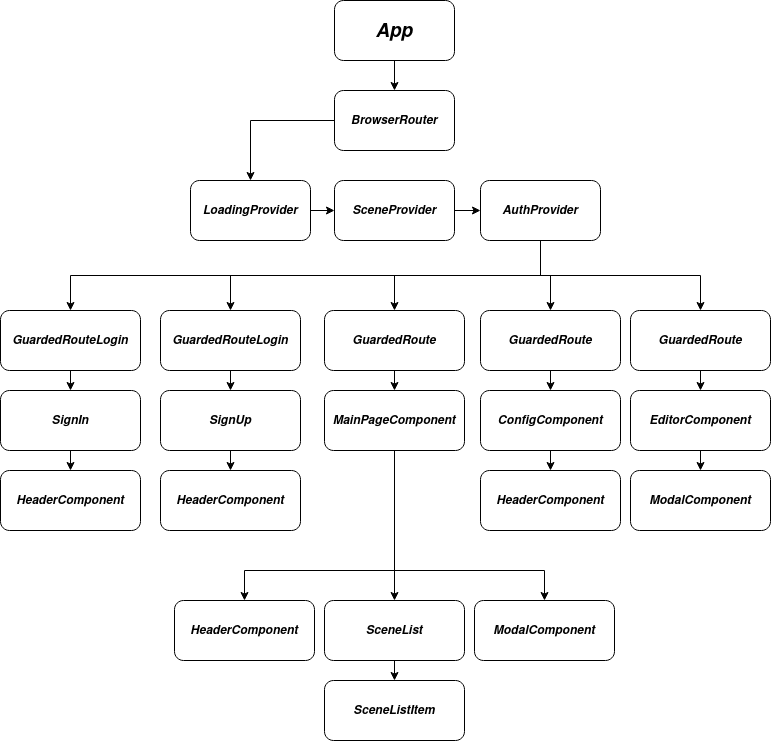
\includegraphics[scale=0.4]{reactdiagram}
    \caption[Diagrama de componentes React de aplicación web]{Diagrama de componentes de React para la aplicación web.}
    \label{fig:reactdiagram}
\end{figure}

El bloque de construcción básico de las aplicaciones en React son los \textbf{componentes}. Estos son elementos funcionales de interfaz, reutilizables, anidables y parametrizables. Se escriben en la extensión de TypeScript \textit{.tsx}, y se encuentran en la carpeta \textit{src/components} del proyecto. Un componente puede ser por ejemplo un botón que haga una acción específica, o la cabecera de una página, un menú desplegable, etc. El corazón de la aplicación se encuentra en el componente \textbf{EditorComponent.tsx}, que gestiona el editor 3D y su interacción con el usuario. Se puede apreciar la estructura de los diagramas del proyecto en la figura \ref{fig:reactdiagram}.

\subsection{Renderización de entorno 3D}

Lo primero que se realizó antes del componente en sí con toda la interfaz, fue implementar el entorno 3D interactuable. Para ello se hizo la clase \textbf{EditorScene.ts}, que hereda de la clase \textit{Scene} de la librería de Three.js. \textit{Scene} se encarga de gestionar la escena entendida como el espacio donde habitan los distintos objetos 3D de la aplicación. En Three.js, los espacios 3D se representan con una estructura de datos en forma de árbol. Los objetos son hijos unos de otros, y el objeto especial \textit{scene} es el nodo raíz. Un objeto es hijo de otro objeto, todas las transformaciones que se apliquen al padre también se efectuarán en el hijo.

Para poder visualizar un entorno 3D de Three.js se necesita un objeto \textit{Scene}, una cámara \textit{PerspectiveCamera} y un renderizador \textit{WebGLRenderer}. La cámara se puede entender conceptualmente como si fuese una real. Es un objeto que está en una posición determinada del espacio 3D y ``grabando'' en una dirección. Se encarga de definir qué parte de la escena es la que se va a ver por pantalla. Esta información se transmite al renderizador, que realiza cálculos para convertir la representación abstracta del espacio 3D a una imagen en dos dimensiones que se puede mostrar por pantalla y que el usuario puede entender. Los tres elementos se inicializan y mantienen desde \textbf{EditorSceneController.ts}. Esta clase hace de interfaz e implementa las llamadas necesarias para que el componente \textit{EditorComponent.tsx} pueda realizar cambios en la escena y cámara a través de su interfaz de usuario.

\subsection{Controles de cámara y selección de objetos}

Para la manipulación de la cámara se adoptaron controles estándares presentes en otros programas de edición: arrastrando con el clic derecho del ratón se rota la cámara sobre un punto, y con la rueda del ratón se desplaza. Así queda el clic izquierdo libre para las interacciones con los objetos.

El usuario debe poder seleccionar un objeto de la escena colocando el ratón sobre él y haciendo clic. Esto le servirá para, una vez elegido un modelo, poder manipularlo moviéndolo, rotándolo o escalándolo sin afectar al resto de objetos de la escena. Esto presenta el problema de cómo saber cual es el objeto que se ha seleccionado. Para ello se utilizó un \textbf{raycaster}. Es un recurso muy usado en la informática gráfica y disponible en la librería de Three.js. Consiste en disparar una suerte de haz o rayo desde un punto de la escena y en una dirección. Este disparo atraviesa los objetos 3D que se encuentra en su camino y devuelve una lista ordenada de los modelos con los que ha colisionado. Para este proyecto se implementó un raycast desde el punto en el que se encuentra la cámara (es decir, la perspectiva del usuario) y en dirección al punto en el que se hace clic. De esta forma el rayo ensarta el punto en el que se ha pulsado, y si había un objeto debajo, colisionará con él. En la clase de raycast que implementa \textit{Three,js} se le debe pasar como parámetro una \textit{Scene} o un \textit{Group}, un objeto especial que tiene como hijos una lista de objetos. El rayo solo detectará colisiones con objetos de dicha lista o que pertenezcan a la \textit{scene}. Aparece así otro problema: si se pasa la \textit{scene} como parámetro detectaría cualquier objeto que haya en esta, no solo los que haya añadido el usuario.

Se debe distinguir entre dos tipos de objetos que se encontrarán en la escena: los dinámicos que los añade el usuario y son interactuables por este, y los estáticos, que se crean al iniciarse el espacio 3D automáticamente y tienen de propósito servir de referencia visual, como por ejemplo un \textit{grid} (figura \ref{fig:grid}) que simboliza dónde está el suelo. Todos estos objetos se deben añadir a la \textit{scene} como hijos de esta usando \textit{scene.add(object)}. Para diferenciar las dos clases de elementos se añade a la escena un \textit{Group} con el nombre de \textbf{liveObjects}. Los modelos introducidos por el usuario serán entonces añadidos como objetos a este atributo, y será el parámetro que se pasará al raycaster para que solo reconozca objetos \textit{dinámicos}, solucionando así el problema de reconocimiento. Para eliminar objetos de la escena simplemente habría que desconectar al nodo hijo correspondiente de \textit{liveObjects}.

\begin{figure}[h]
    \centering
    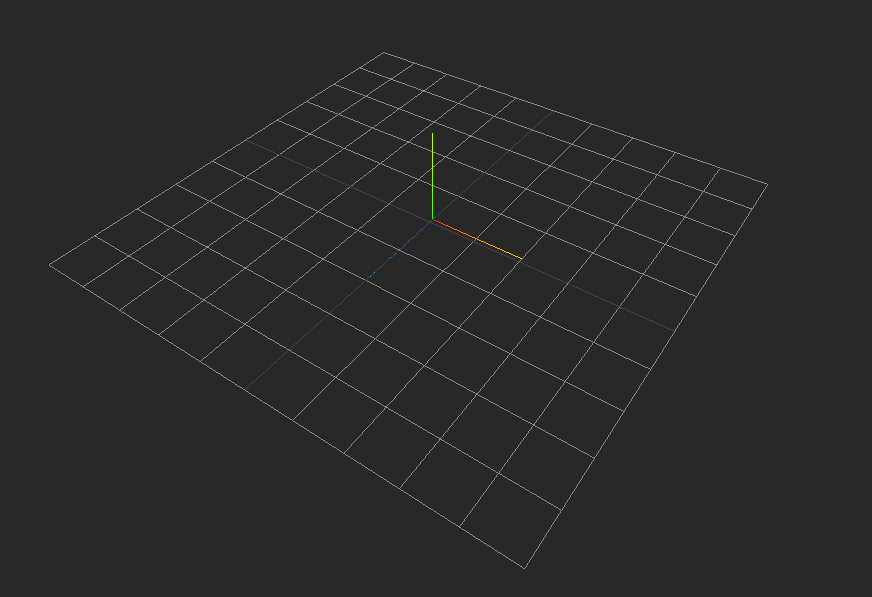
\includegraphics[scale=0.30]{grid}
    \caption[Grid del editor de escenas]{Grid del editor de escenas para tener de referencia como suelo.}
    \label{fig:grid}
\end{figure}

Sin embargo, esto ocasiona otro problema. Se ha comentado anteriormente que un objeto 3D puede ser hijo de otro, y esto es muchas veces el caso con los modelos que se pueden encontrar en la web. Es muy probable que si por ejemplo se carga en la escena a \textit{robot.glb}, este esté hecho de múltiples objetos 3D. Uno de estos podría ser su brazo, su cabeza o su cuerpo. Esto es problemático porque si fuera el caso y se hace clic en el brazo del robot con la intención de seleccionar el modelo entero, el raycaster solo devolverá información sobre el nodo hijo. Para solucionar esto se hizo uso del atributo \textbf{name} que tienen todos los \textit{Object3D} de Three. Este atributo es un string con el que se puede asignar un nombre al objeto. 

En la función que añadía los objetos del usuario al grupo de \textbf{liveObjects}, se pasó a etiquetar los \textit{name} de todos los elementos como ``alive''. De esta forma, cuando se obtiene un nodo hijo de un modelo, se puede ir recorriendo el padre de cada nodo hasta encontrar uno cuyo \textit{name} sea igual a ``alive''. Aquí pararía la búsqueda, ya que, de seguir ascendiendo por sus padres se llegaría a la \textit{scene}, el nodo raíz. Tras esto el raycaster sería capaz de detectar qué objeto selecciona el usuario. 

El usuario debe ademaś tener la posibilidad de hacer una selección múltiple de objetos para que las transformaciones que se apliquen afecten a todos simultáneamente. Para ello se hará clic en otro objeto mientras se pulsa la tecla \textit{Control}. Este es un esquema de control usado tanto en software del sector como en los gestores de archivos de los sistemas operativos, es un gesto muy reconocido. Si ya había un objeto seleccionado y el usuario está pulsando la tecla mientras elige otro objeto, este se añadirá a un array de objetos seleccionados.

\subsection{Transformación de objetos}

Una vez está resuelta la selección de objetos es necesario implementar la forma en la que el usuario comanda las transformaciones que se aplican sobre estos. Se usarán los \textbf{gizmos} comentados en el anterior capítulo para ello. Three.js incorpora \textit{gizmos} bajo la clase \textit{TransformControls}. Esta clase cuenta con tres modos: translación, rotación y escalado. La clase puede ``engancharse'' a un objeto que se le pase como argumento. Una vez hecho mostrará el gizmo correspondiente en función del modo actual superpuesto sobre el objeto. El usuario podrá hacer clic directamente sobre él para manipular el objeto.

Aquí apareció otro problema. La clase solo soporta un objeto ``enganchado'' al mismo tiempo, por lo que en el caso de tener varios objetos seleccionados no se podrían modificar todos. La primera solución que se intentó dar a esto fue hacer a todos los modelos seleccionados hijos de un nodo temporal vacío el cual se asignaría al \textit{TransformControls}. Esto no funcionó debido a que las transformaciones en \textit{Three.js} son locales respecto al padre del objeto. Es decir, si se aglutinan los objetos seleccionados en un nodo y se mueven dentro de ese nodo, cuando se devuelven a la escena regresan a su lugar de origen. Esto se arregló con un \textit{dummie}, que es un objeto invisible que sirve como apoyo para hacer ciertas operaciones en la informática gráfica. En este caso, cuando se inicia una selección múltiple se crea un \textit{dummie} en el origen de coordenadas y se asigna a los \textit{TransformControls}. En cada frame, se comprueba cuanto se ha modificado su posición, rotación o escalado y se aplica esa misma variación a todos los objetos de la lista de seleccionados. Con esto la funcionalidad estaba lista.

\subsection{Reproducción de animaciones}

Algunos modelos 3D incluyen animaciones. El usuario cuenta con una opción en su interfaz para poder reproducir la escena, y con ello las animaciones de todos los objetos que se encuentren en esta. Los \textit{Object3D} de Three soportan animaciones, y para poder reproducirlas se hace uso de la clase \textbf{AnimationMixer}. Esta recibe un objeto como parámetro y automáticamente extrae toda la información relativa a sus animaciones. Cada animación está identificada con un string que le da nombre como podrían ser ``Death'', ``Walk'' o ``Run''. Desde \textit{AnimationMixer} se invoca a la función \textit{clipAction(animacion)} y se obtiene un objeto de tipo \textit{AnimationAction}. Desde este último se puede ordenar a las animaciones que se reproduzcan o se detengan.

Como el usuario necesita tener la capacidad de elegir una animación concreta de entre las muchas que puede tener un modelo para que se reproduzca, se necesita registrar en algún sitio cuál es la seleccionada. Para ello se empleó el atributo \textbf{userData} de \textit{Object3D}. Este es un objeto genérico JavaScript en el que se puede definir multitud de datos auxiliares relacionados con el modelo. Se define entonces el atributo \textbf{animationIndex}, un número entero que va de 0 a \textit{n-1}, siendo \textit{n} el número de animaciones que posee ese objeto. Cuando se quiere reproducir las animaciones en la escena, para cada objeto se crea un \textit{AnimationAction} con el índice actual del objeto y se llama al método \textit{animationClip.play()}. Cuando se quiera detener la animación, se ejecutará \textit{animationClip.reset()} para que los modelos vuelvan a su estado inicial y \textit{animationClip.stop()} para que se detengan.

\subsection{Exportación y carga de escenas}

Para la carga de modelo en la aplicación se parte desde la base de que el usuario tiene acceso a archivos \textit{.glb} de forma local en su dispositivo, que lo ha cargado desde la interfaz de la aplicación y se guarda en un objeto JavaScript \textit{File} en la caché y con una url temporal para acceder al recurso. Para cargar el modelo se hará uso de la clase de Three.js \textbf{GLTFLoader}, que permite convertir un \textit{File} en \textit{Object3D} a partir de su \textit{URL}. Después se añadiría el \textit{Object3D} como hijo a \textit{liveObjects} y ya sería visible en la escena.

Para la exportación de la escena es estrictamente necesario encontrar la forma de convertirla en un archivo único \textit{.glb}. Para ello se empleó la clase de Three.js \textbf{GLTFExporter}. Esta recibe como argumento un objeto o grupo de objetos y los convierte a un archivo \textit{.gltf}, o \textit{.glb} si se especifica el parámetro \textit{binary} como verdadero. Como resultado se obtiene un buffer con un array de datos \textit{raw}, es decir binarios. Estos datos pueden utilizarse para crear un objeto \textit{Blob} que se puede descargarse como fichero a través del navegador. Solo es necesario entonces pasarle al \textbf{GLTFExporter} el grupo de objetos vivos (los que introdujo el usuario) \textit{liveObjects} y la clase hará el resto del trabajo. El archivo resultante no solo contendrá el modelado sino las animaciones de todos los objetos de la escena.

Con lo desarrollado hasta ahora sería posible descargar la escena al ordenador como usuario, pero existe un segundo caso en el que se requiere exportar una escena: guardarla en el servidor. Se necesita establecer la forma en la que se van a almacenar los datos de la escena como los objetos que contiene, su posición, rotación y escalado, su índice de animación activa, su lista de animaciones, etc. Para ello se contemplaron dos opciones:

\begin{itemize}
    \item \textbf{Archivo binario único}: Los modelos se exportarían a un fichero similar al descargable por el usuario en el que la escena se convierte en un único modelo. El archivo sería lo que se almacenaría en la base de datos, conteniendo este toda la información sobre los modelos que se tienen y su estado actual. Esto requeriría que fuera posible cargarlo a posteriori en el editor, separando todos los modelos para añadirlos de manera individual a la escena y que conserven su independencia.
    
    \item \textbf{JSON}: Se guardaría en la base de datos una copia de cada modelo en la escena. Adicionalmente, se guardaría un archivo JSON en el que se describen uno por uno la posición, translación y escalado de cada objeto, además de otros parámetros como el \textit{animationIndex} para cada uno de ellos si es que tienen.
\end{itemize}

La primera opción era la preferible, ya que era una solución mucho más simple y elegante, tanto a la hora de empaquetar los datos como de almacenarlos en la base de datos (solo se guardaría un único archivo con toda la información). Por suerte, cuando \textit{GLTFLoader} carga un archivo \textit{.glb} conserva toda la estructura de nodos del objeto original. Tras hacer algunas pruebas se comprobó que \textit{GLTFExporter}, al recibir un grupo de objetos como entrada para exportar una escena, los emparenta a todos a un nodo raíz. Sabiendo esto se tiene la certeza de que al cargar un archivo previamente exportado desde la aplicación, los hijos del nodo raíz serán exactamente todos los objetos interactuables de la escena. Se implementó una función \textit{loadScene} que recorría la lista de hijos del archivo \textit{.glb} recibido y los añadía uno a uno a la escena.

Un detalle que tuvo que tenerse en cuenta fue que \textit{GLTFExporter} al empaquetar la escena almacena todas las animaciones de los objetos en un único array en el nodo raíz en lugar de en sus respectivos nodos. Al cargar el archivo posteriormente no hay forma de saber qué animaciones pertenecían a cada objeto para poder asignárselas. Para solucionar esto, antes de añadir un objeto a la escena se crea un array de datos en el atributo \textit{userData} del objeto conteniendo el nombre de todas las animaciones del modelo. Así, al cargar cada objeto luego, se podría comprobar en la lista general de animaciones del \textit{.glb} y añadir a \textit{animations} las que coincidan en nombre.

\subsubsection{Conflicto entre animaciones}

Llegados a este punto la escena se cargaba correctamente pero surgió un problema derivado de las animaciones de los archivos exportados. Para explicar la resolución es necesario aclarar algunos detalles sobre las animaciones en Three.js.

Como se muestra en la figura \ref{fig:}, las animaciones de un modelo se guardan en un atributo de \textit{Object3D} llamado \textbf{animations}, un array de objetos \textit{AnimationClip}. Estos objetos a su vez tienen entre sus atributos un array de \textit{KeyframeTrack}, objetos que almacenan secuencias de \textit{keyframes} con información sobre las transformaciones que realiza la animación a un objeto. ¿Cómo saben estas estructuras de datos a qué nodo se deben aplicar estos movimientos? \textbf{A través del \textit{name}} de los \textit{Object3D} de la escena. En resumen: las animaciones saben qué nodo deben mover porque los identifican con su nombre.

\begin{figure}[h]
    \centering
    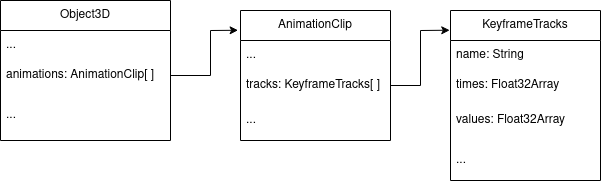
\includegraphics[scale=0.55]{animationesquema}
    \caption[Esquema de estructura de datos para animaciones]{Esquema de las estructuras de datos de \textit{Object3D}, \textit{AnimationClip} y \textit{KeyframeTrack} para la reproducción de animaciones.}
    \label{fig:animationesquema}
\end{figure}

Por otro lado, \textit{GLTFExporter} al exportar la escena tiene un comportamiento muy relevante para este caso: \textbf{si dos nodos tienen el mismo nombre, modifica uno de ellos}. Por ejemplo, si hubiera dos nodos llamados \textit{hand}, al segundo lo renombraría como \textit{hand\_1}.

Sabiendo esto se puede describir el verdadero problema: \textbf{si dos modelos tienen una animación apuntando al nodo \textit{hand}, solo se moverá el primer objeto}, ya que las animaciones del segundo apuntarán también a \textit{hand}, pero el nodo equivalente del segundo modelo en realidad se llama \textit{hand\_1} y no se ve afectado por la animación. Este fue un punto crítico del desarrollo, ya que de arreglar esto dependía poder ahorrar luego mucho tiempo de en el backend y simplificar el funcionamiento del sistema. 

Para solucionarlo se hizo uso de otro atributo de \textit{Object3D}, el \textbf{id}, una variable numérica que identifica un objeto en una escena. Al cargar nuevos objetos en la escena, se comprueba si coinciden sus nodos con los de otro objeto. En caso afirmativo, se concatena el \textit{id} del objeto recursivamente a todos sus nodos hijos, y luego se hace lo mismo para el array de \textit{animations}, para que los \textit{KeyframeTrack} apunten a los nodos con el nombre cambiado. Si el \textit{id} de un objeto repetido es \textit{23}, su nodo hijo \textit{hand} pasará a llamarse \textit{23\#hand}, evitando así todos los conflictos que puede generar el \textit{GLTFExporter}.

Con esto la exportación y carga de escenas es perfectamente funcional para cualquier caso, y podrá ser empleada para almacenarse en la base de datos como un único archivo.

\subsection{Reproducción de audios}

Los audios asociados a las escenas se manejan desde \textbf{EditorSceneController.ts}. La clase tiene el atributo \textit{audio} de tipo \textit{HTMLAudioElement}, que permite reproducir audios cargados por \textit{url}. Como se mencionó antes, se da por supuesto que el usuario carga un archivo de audio compatible y este se almacena en la caché accesible desde una url. Con la función \textit{loadAudio} se crea el objeto que gestionará su reproducción con los métodos \textit{playAudio} y \textit{stopAudio}.

\subsection{Interfaz del componente editor}

Ahora se discutirá el \textbf{EditorComponent.tsx} en sí, el componente que contiene la interfaz del editor y realiza las llamadas pertinentes a \textit{EditorSceneController} en función del input del usuario.

Todo lo que a la interfaz se refiere se diseñó previamente en \textbf{Figma}\cite{figma} (figura \ref{fig:editorfigma}), un software para \textit{mockups} de interfaces de usuario. Todos los elementos como botones, selectores y cajas de texto se implementaron usando \textit{MUI Core}, una librería de React para la creación de interfaces de usuario. Ofrece todos los bloques fundamentales que pueden necesitarse para la construcción de aplicaciones web y además adopta \textit{Material}, unas directrices de diseño lanzadas por Google para interfaces web y móviles. Es lo mismo que se acabaría empleando en la aplicación Android, así que de entre todas las librerías que existían con el mismo propósito, se eligió esta para unificar en la medida de lo posible el estilo de las aplicaciones web y de móvil del proyecto.

\begin{figure}[h]
    \centering
    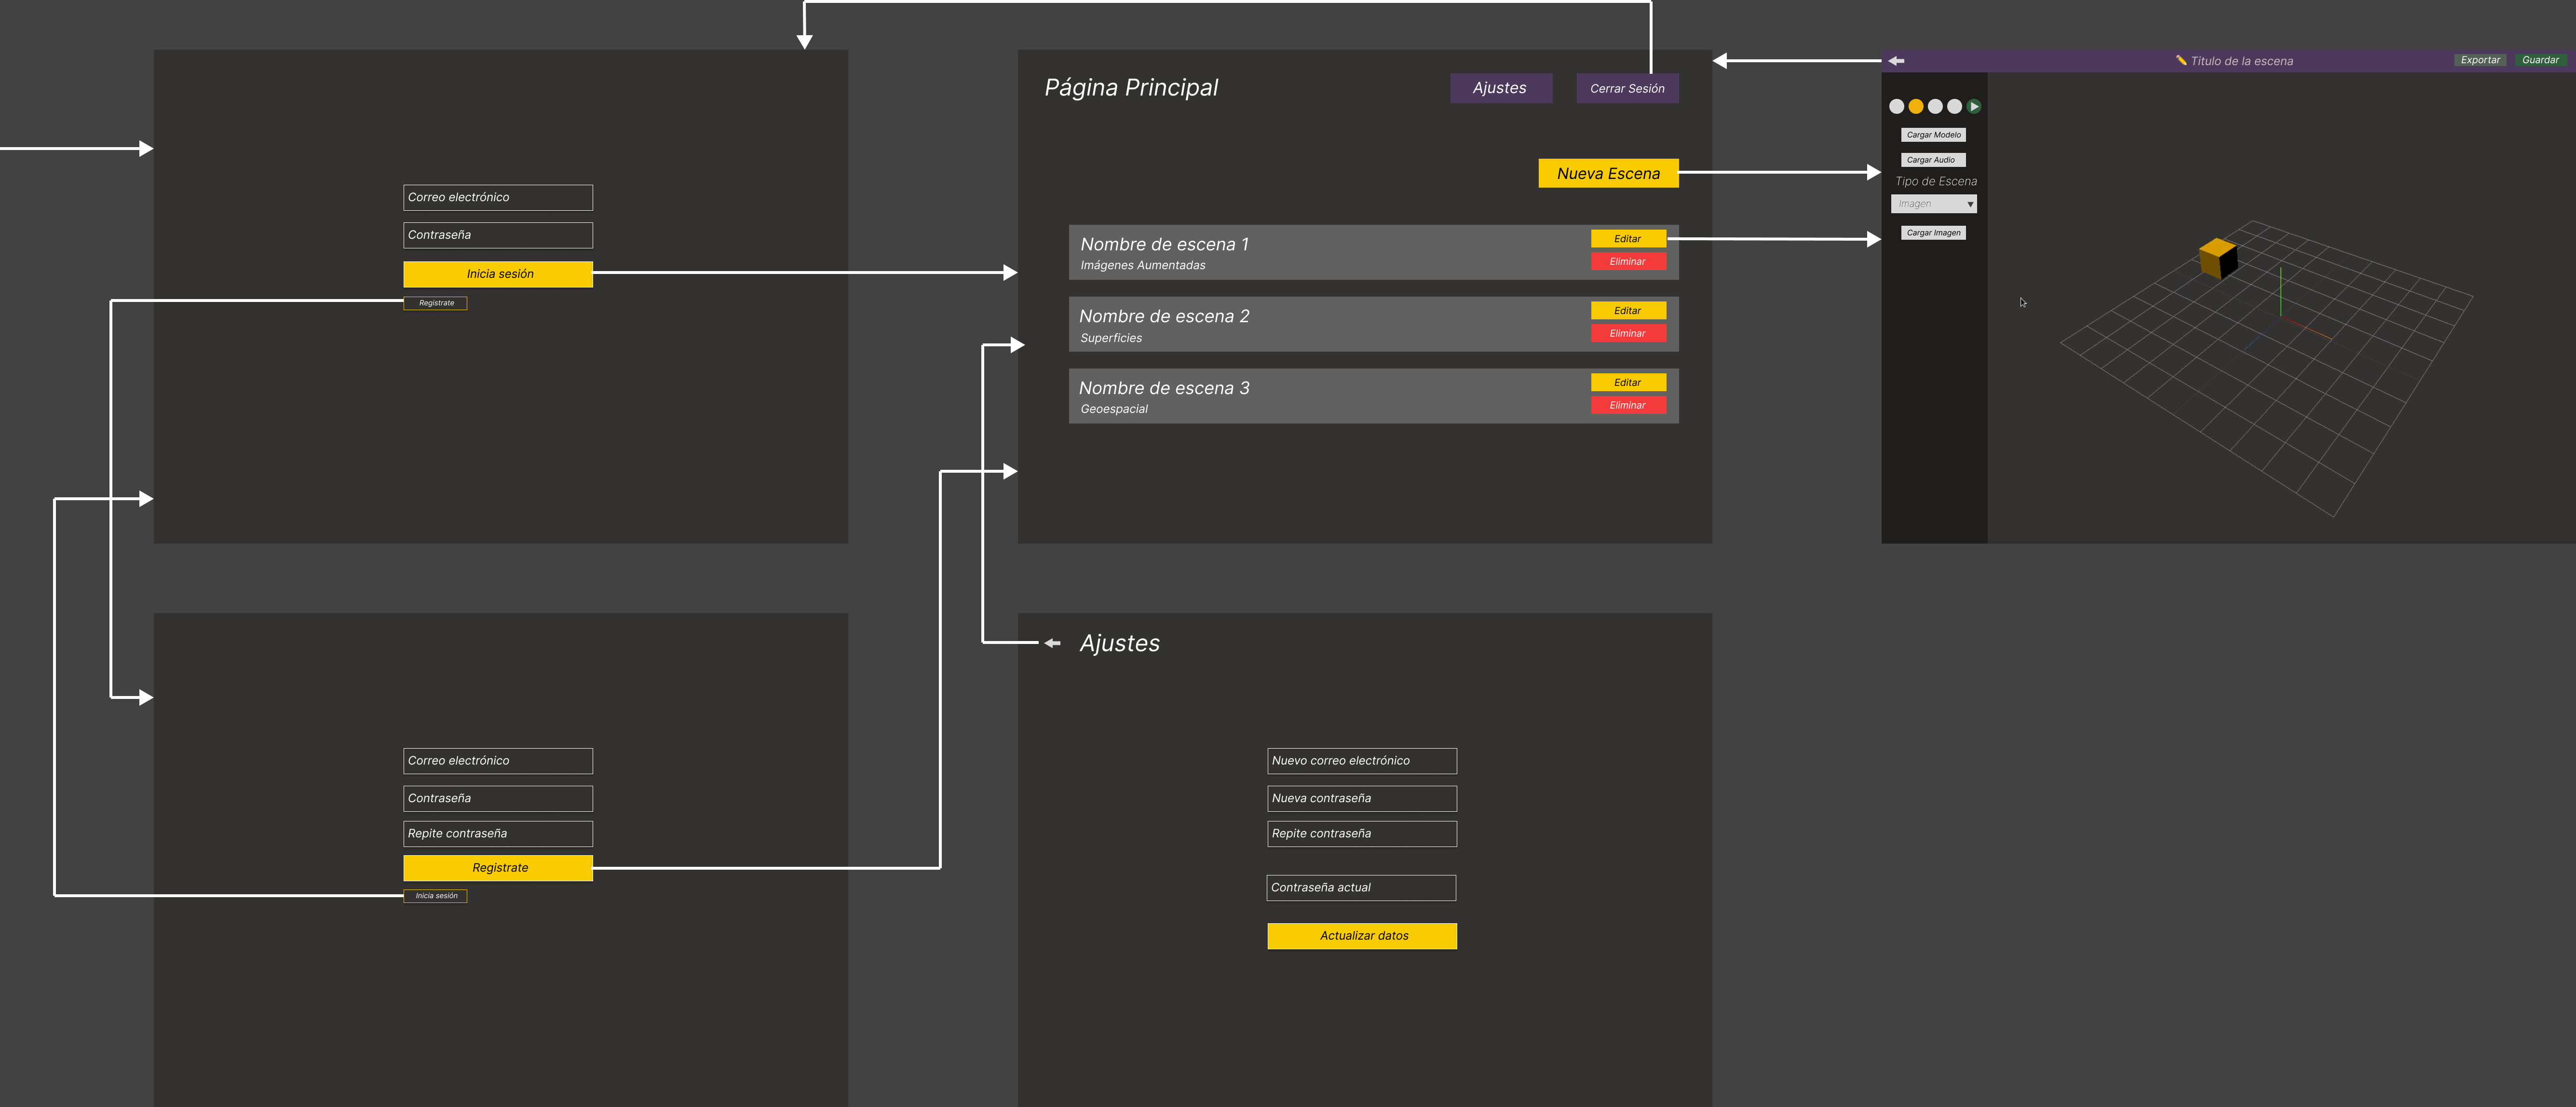
\includegraphics[scale=0.07]{editorfigma}
    \caption[Mockup de la UI de la aplicación web]{Mockup de la UI de la aplicación web realizado en \textit{Figma}}
    \label{fig:editorfigma}
\end{figure}

La interfaz (figura \ref{fig:editorfinal}) se dividió en tres secciones:

\begin{enumerate}
    \item La barra superior. Aquí se encontrarían los botones para exportar y guardar la escena, un cuadro de texto para introducir el nombre de la misma, y un botón para volver al anterior menú.
    \item La barra lateral, un panel de control con todas las opciones para configurar la escena AR.
    \item El \textit{canvas}, todo el espacio sobrante entre las dos barras donde se renderizaría el entorno 3D del editor.
\end{enumerate}

\begin{figure}[h]
    \centering
    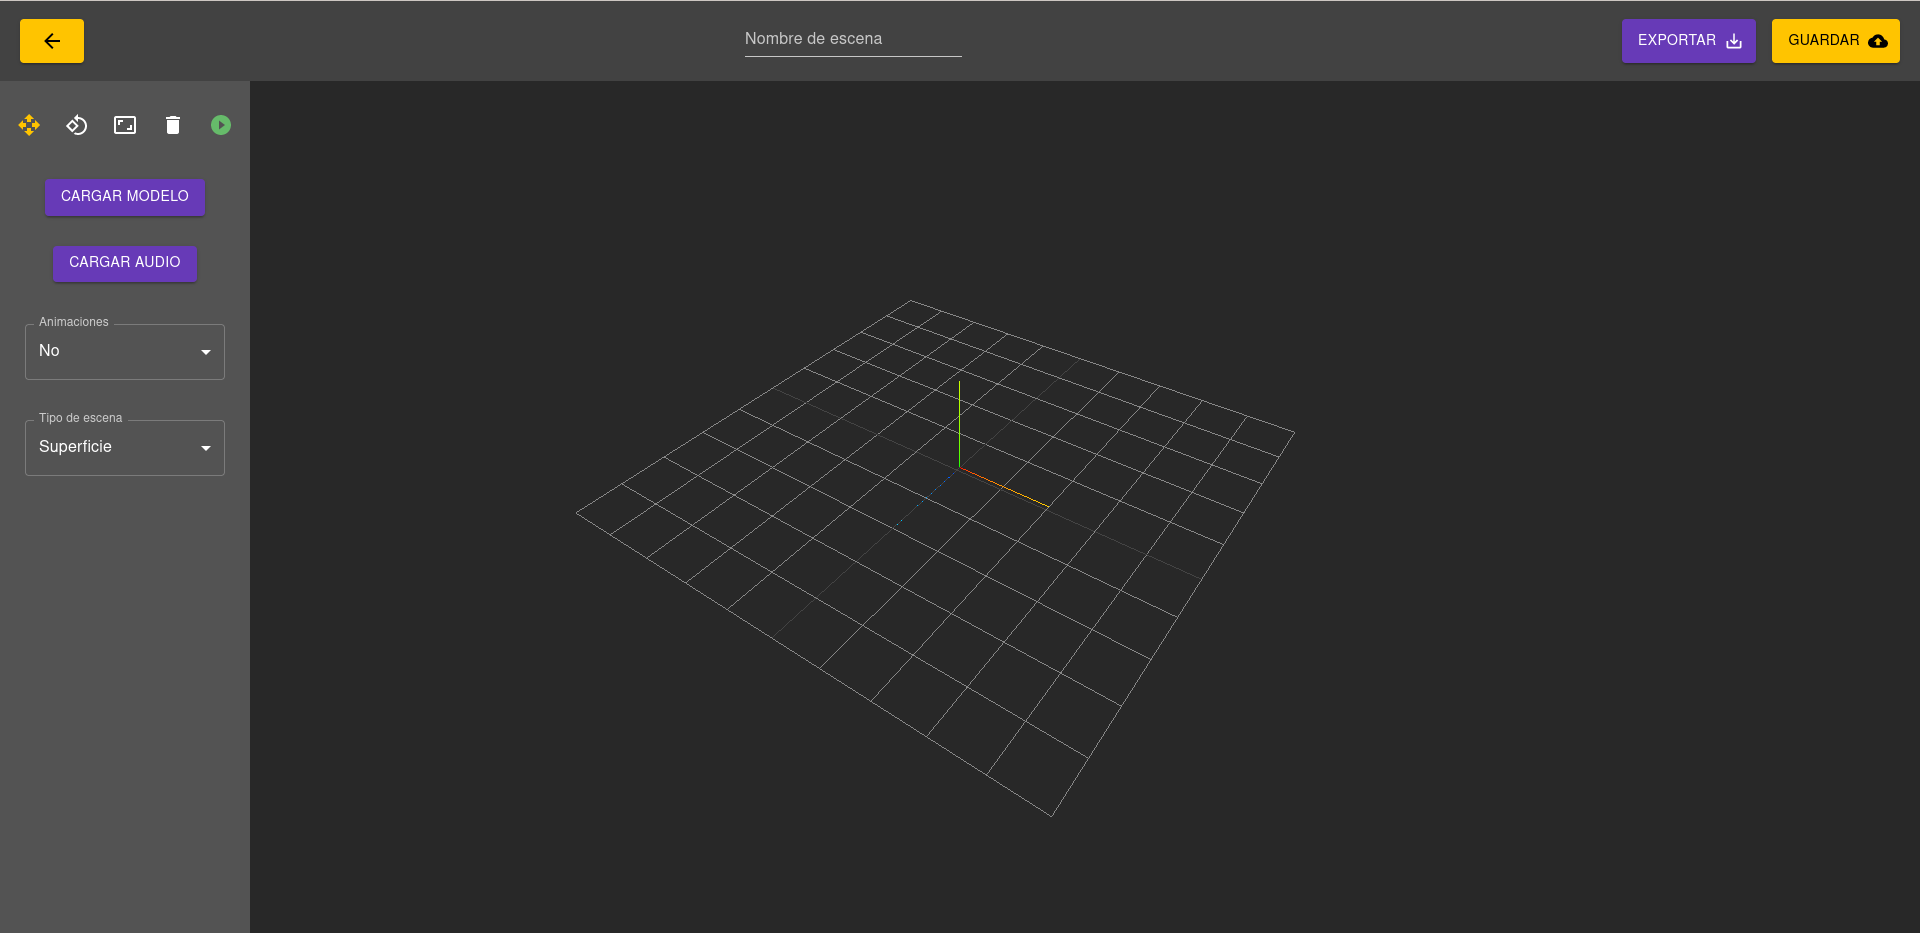
\includegraphics[scale=0.19]{editorfinal}
    \caption[Interfaz de usuario para el editor de escenas]{Interfaz de usuario final para el editor de escenas.}
    \label{fig:editorfinal}
\end{figure}

En este componente y en el resto de la aplicación se emplean los llamados \textit{hooks} de React. Estas son unas funciones JavaScript que entre otras cosas permiten dotar de estado a un componente, ya que de normal no tienen. Por ejemplo, si se quisiera hacer un contador de clics, este tendría que tener el número de pulsaciones actual guardado. Esto es posible gracias al hook de \textbf{useState}, que permite almacenar variables persistentes entre distintas renderizaciones de un componente. En este proyecto se utiliza entre otras cosas para almacenar la instancia de \textit{EditorSceneController} que se crea al iniciar una escena por primera vez y renderizarlo en el \textit{canvas}.

Para el panel de control lateral se tienen las siguientes utilidades:

\begin{itemize}
    \item \textbf{Botones de herramientas}: Con estos botones se puede elegir qué herramienta utilizar para manipular la escena. Dependiendo de cual se tenga escogida cambiará la forma de manipular un objeto. Cambiará de color en función de la herramienta seleccionada. Se cuenta con las siguientes:
        \begin{itemize}
            \item Translación: Con esta herramienta aparecerá un \textit{gimzo} de desplazamiento en los objetos seleccionados, con el que se podrá mover de posición.
            \item Rotación: De forma similar a la anterior herramienta, con esta se pueden rotar objetos.
            \item Escalado: Con esta herramienta se pueden hacer los objetos más grandes o más pequeños en cualquier eje de coordenadas.
            \item Papelera: Con esta herramienta seleccionada, los objetos clicados desaparecerán de la escena.
        \end{itemize}

    \item \textbf{Botón de play}: Previsualiza la escena en el editor. Reproduce las animaciones de los modelos de la escena si estos tuvieran y la opción de animaciones estuviera activa y/o el audio si hubiera.
    \item \textbf{Cargar modelo}: Abre el navegador de archivos del dispositivo para seleccionar un archivo \textit{.glb} y añadirlo a la escena. Opcionalmente, el usuario puede cargar modelos arrastrando el archivo a la ventana del navegador.
    \item \textbf{Cargar audio}: Abre el navegador de archivos del dispositivo para seleccionar un archivo de audio para asociarlo a la escena. Al tener algún archivo cargado aparece una ``x'', que si se pulsa eliminará el audio de la escena.
    \item \textbf{Animaciones}: Menú desplegable para establecer si reproducir o no las animaciones de los modelos.
    \item \textbf{Tipo de escena}: Menú desplegable para elegir el tipo de escena. Dependiendo del tipo elegido aparecerá abajo una opción adicional para añadir configuración adicional necesaria:
        \begin{itemize}
            \item Imágenes aumentadas (Marcador): Aparece un botón para cargar una imagen. Esta imagen se pasará a \textit{EditorScene} como objeto \textit{File} y será cargada como textura plana en el suelo de la escena para tenerla como referencia.
            \item Geoespacial: Aparecen tres campos numéricos para introducir la latitud, longitud y altura a la que se desea que aparezca la escena.
            \item Superficie: No se muestra ningún menú adicional.
        \end{itemize}
\end{itemize}

\subsection{Carga de archivos}

La carga de archivos como modelos, audio o imagen se gestiona a través de la función \textit{handleLoad}. Esta se llama en un evento \textit{onChange} para los elementos HTML asociados a los botones de carga. Este evento se activará cada vez que se cargue un nuevo archivo y lo pasará como parámetro en forma de objeto \textit{File}. Ahí se comprueba si es uno de los archivos soportados (\textit{.glb} para los modelos, \textit{.mp3} o \textit{.ogg} para los audios y \textit{.jpg}, \textit{.png} o \textit{.svg} para las imágenes). Si la extensión del archivo cae en alguna de estas categorías, se crea una \textit{URL} temporal para acceder al objeto en caché y se llama a la función de \textit{EditorSceneController} correspondiente: \textit{loadModel}, \textit{loadAudio} o \textit{loadImage}. La clase se encarga de gestionar esas entradas como se ha visto anteriormente.

\subsection{Gestión de evento asíncrono en el guardado}

Para guardar la escena se tienen en la esquina superior derecha dos botones, uno para descargar la escena como modelo (Exportar) y otro para guardarlo en el servidor (Guardar). Se debe tener en cuenta que la función de \textit{EditorScene} que convierte la escena en modelo, \textit{exportScene}, es asíncrona. En el caso de \textit{Exportar} no hay ningún problema, ya que cuando termina el proceso no hay que hacer nada más, es descargado por el navegador. Sin embargo en el caso de \textit{Guardar} surgía un inconveniente. Para enviar el archivo a la base de datos se necesita esperar a que este termine. Por cómo funciona \textit{GLTFExporter}, el resultado de la función \textit{parse} (la que se usa para hacer la conversión) no puede ser devuelto por la función donde se ejecuta ya que está dentro de un contexto de función distinto. Introducir en la clase de \textit{EditorScene} código para hacer peticiones HTTP al backend era posible, pero una solución poco elegante, ya que, ese no es el propósito de la clase.

Se optó por hacer en \textit{EditorScene} una versión clónica de \textit{exportScene()} llamada \textit{getBlob(upload: (blob: Blob) => void)}. Esta recibe como argumento una función, \textit{upload} que a su vez recibe como argumento un \textit{Blob} (equivalente a \textit{File}). Esta función es definida en \textit{EditorComponent} y llamada dentro del contexto de finalización de las labores de \textit{GLTFExporter}. Contiene el código para realizar las peticiones HTTP para enviar la escena al backend. En resumen, desde \textit{EditorScene} se ejecuta código de \textit{EditorComponent} para comunicarse con el servidor cuando la escena está lista para ser enviada.

\subsection{Navegación entre distintas páginas}

React es una librería y no un framework. Por ello, de base solo tiene capacidad para soportar \textit{single page applications}. Sin embargo, se necesitaba crear una interfaz con distintas páginas: inicio de sesión, configuración de perfil, selección de escena y editor. Para ello se empleó \textbf{React Router}\cite{reactrouter}, una librería que permite definir distintas páginas cada una asociada a una \textit{URL} distinta (\textit{/login}, \textit{/config}, etc.).

Las páginas con las que cuenta la aplicación son las siguientes:

\begin{itemize}
    \item \textbf{MainPageComponent} \textit{/}: Página principal de los usuarios conectados. Se muestra el listado de escenas para poder editarlas o eliminarlas además de opciones para iniciar una nueva escena, cerrar sesión o cambiar credenciales.
    \item \textbf{SignInComponent} \textit{/login} y \textbf{SignUpComponent} \textit{/register}: Páginas para crear una cuenta de usuario e iniciar sesión.
    \item \textbf{ConfigComponent} \textit{/config}: Menú para actualizar las credenciales del usuario.
    \item \textbf{EditorComponent} \textit{/editor}: Editor de escenas.
\end{itemize}

\subsection{Rutas protegidas}

Al ser accesible cualquier página de la aplicación a través de su \textit{URL} surgía un nuevo problema. En el planteamiento propuesto, el usuario debía registrarse o iniciar sesión antes de poder acceder a páginas como su lista de escenas o el editor. Se necesitaba entonces \textit{proteger} las páginas sensibles al inicio de sesión bajo la condición de que se hubiera realizado. Esto se implementó con el componente \textbf{GuardedRoute.tsx}. Como se mencionó anteriormente, los componentes en React pueden estar anidados. Se anidaron todas las páginas sensibles dentro de un \textit{GuardedRoute} cada una. Este se encargaría de comprobar si existe una sesión iniciada. En caso afirmativo renderiza a su hijo, la página protegida. Si no, redirige la aplicación a \textit{/login} para que el usuario pueda iniciar sesión. Para las páginas de inicio de sesión de registro se siguió el razonamiento contrario: si se accede a estos con una sesión iniciada, redirige la aplicación a la página principal.

\subsection{Contextos compartidos}

En \textit{React} cada componente tiene su propio contexto. Las funciones y variables que se declaran dentro de uno solo pueden ser accedidos por él mismo, a menos que un padre las pase como argumento a un hijo, en cuyo caso este sí  podría usarlas también. Esta solución es un poco rudimentaria si se va a necesitar más que una variable puntual, mucho más si hay componentes anidados a varios niveles y el nodo del fondo necesita hacer uso de algún elemento del padre de todos.

Esto fue un problema cuando se trataba con la gestión del usuario activo y llamadas a la API. El usuario activo se almacena en un objeto de la librería de \textit{Firebase} (se explicará en siguientes apartados). Este objeto debía instanciarse una vez y llamarse desde cualquier punto de la aplicación, lo cual era un problema por lo comentado sobre los contextos. Se tendría que pasar este objeto a cada elemento de la página que lo necesitase por parámetros, cosa que no era muy elegante.

Para solucionarlo se emplearon los \textit{createContext} de React. Estos permiten definir unos componentes especiales cuyos descendientes tienen acceso a las variables y funciones declaradas en el padre. \textit{userController} y \textit{sceneController} se crearon para manejar respectivamente las llamadas de usuarios y escenas. Tienen como hijos al resto de los componentes de la aplicación, por lo que se pueden llamar desde cualquier sitio. Además, encapsulan las funciones de comunicación con el servidor, por lo que si en algún momento se fuera a cambiar el backend del sistema solo habría que reescribir estos archivos.

\subsection{Animación de carga}

Existían muchos momentos en la aplicación que suponían una espera para el usuario, como por ejemplo cuando se obtiene el listado de escena, cuando se carga un modelo o al guardar la escena en el servidor. Para hacer saber al usuario que se están haciendo operaciones y la aplicación está reaccionando a sus órdenes se añadió una animación de carga de la librería de \textit{react-spinners}\cite{reactspinners}. Se creó un componente encargado de renderizar esta animación en el centro de la pantalla. En lugar de incluir este componente en cada página que necesitara de un proceso de carga, se introdujo un nuevo \textit{context} de React que envolvía a toda la aplicación, haciendo que desde cualquier punto se pudiera manipular una variable booleana que activaba o desactivaba la animación de carga.

\subsection{Mensajes de incidencia y avisos}

Se introdujeron mensajes en las páginas de inicio de sesión, registro y cambio de datos para alertar al usuario el motivo del error a la hora de realizar una operación no exitosa. Por ejemplo contraseña o correo incorrecto, clave poco segura, correo inválido o ya registrado, etc. También se añadieron mensajes de confirmación en forma de \textit{modales} en acciones irreversibles como al eliminar una escena (\textit{¿seguro que desea eliminarla?}) o al abandonar el editor durante la creación de una escena (\textit{¿seguro? Se eliminarán los cambios no guardados}).

\subsection{Dispositivos no soportados}

Al ser una aplicación web, puede accederse desde cualquier navegador, incluidos \textit{smartphones}, los cuales cuentan con una pantalla reducida y controles táctiles que hacen que el editor no sea manejable desde ahí. Esto no es un inconveniento porque no se diseñó con estos dispositivos en mente, pero si algún usuario entrara desde uno y viera que al interfaz no se adapta a la pantalla y los controles fallan, le resultaría frustrante. Es por eso que se optó por una solución vista en \textit{Onirix Studio}\cite{onirix}. Al detectar que la aplicación se muestra en un dispositivo o ventana demasiado pequeña, se superpone un mensaje con un aviso para que el usuario sepa que la aplicación debe ser accedida desde un ordenador (figura \ref{fig:warning}). Este mensaje bloquea el resto de la aplicación.

\begin{figure}[H]
    \centering
    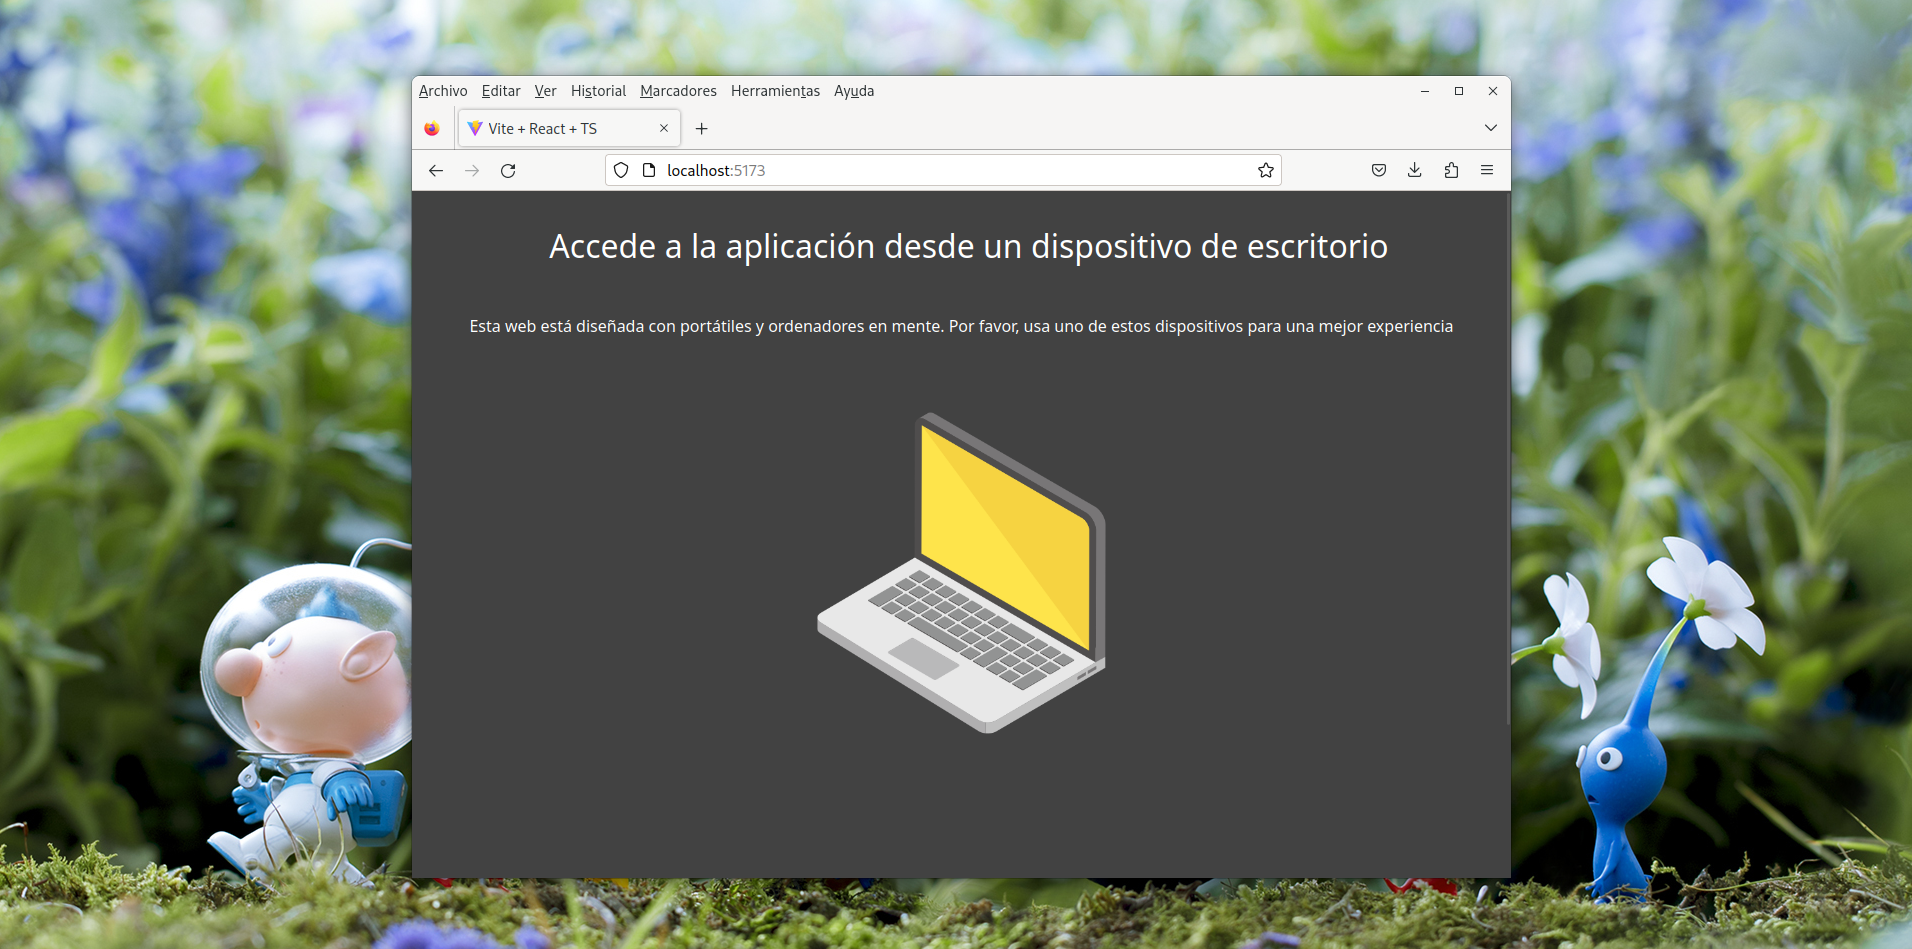
\includegraphics[scale=0.20]{warning}
    \caption[Mensaje de advertencia para dispositvos no soportados]{Si el usuario entra en la app desde un dispositivo no soportado, mostrará este mensaje.Icono sacado de \url{https://www.flaticon.com/authors/vectorsmarket15}.}
    \label{fig:warning}
\end{figure}


\section{Reproductor de escenas Android}

La aplicación Android se compone de tres elementos básicos: una página de inicio de sesión, una página con el listado de las escenas creadas por el usuario activo, y el visor de Realidad Aumentada en función de la escena seleccionada. Se planteó también en un principio una página de registro de usuario pero se descartó debido a que si una persona accedía al sistema por primera vez desde esta app no tendría ninguna escena para reproducir. Por tanto, el registro de usuarios se mantendría únicamente en el editor web. Antes de comenzar con la programación se realizaron diseños para las distintas páginas de la aplicación y la navegabilidad entre estas. Estas páginas reciben el nombre de \textit{actividades} en Android Studio y se representan con una clase Kotlin y un archivo \textit{XML} para la interfaz. En la figura \ref{fig:diagramaAndroid} se puede ver un diagrama de \textit{actividades}.

\begin{figure}[h]
    \centering
    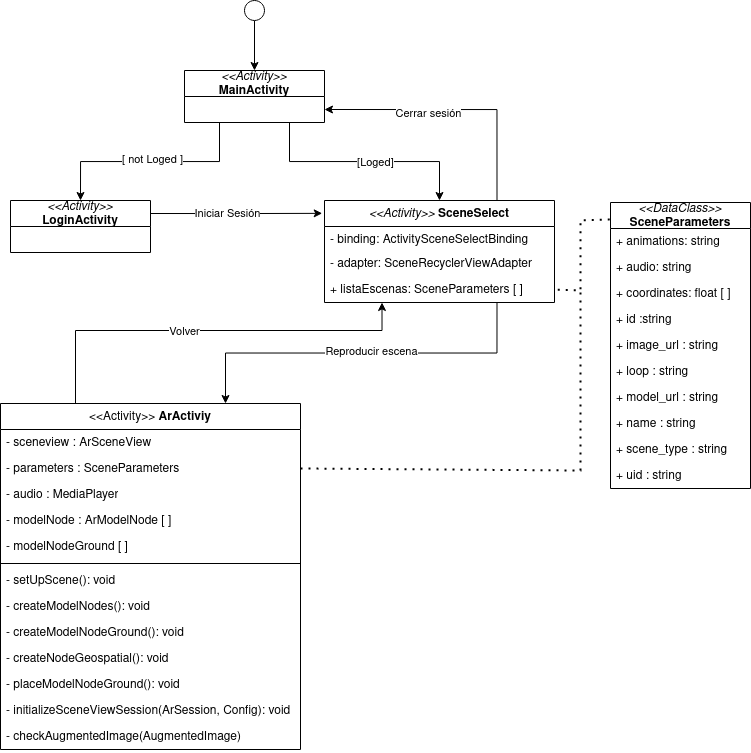
\includegraphics[scale=0.25]{diagramaAndroid}
    \caption[Diagrama de actividades Android Studio]{Diagrama de Actividades para el proyecto de Android Studio.}
    \label{fig:diagramaAndroid}
\end{figure}

\subsection{Archivo de configuración de escena}

Lo primero que hubo que definir es la estructura de datos con la que se representarían las escenas. Este sería el formato usado tanto para almacenarlos en memoria como en la base de datos. Debido a que la base de datos de \textit{Firebase} funcionaba con objetos JSON se decidió que este fichero sería la forma de codificar las escenas. A continuación se tendría que decidir qué campos tendría que tener el archivo. Se llegó a la siguiente lista:

\begin{itemize}
    \item \textbf{name} \textit{(string)}: Nombre de la escena.
    \item \textbf{uid} \textit{(string)}: Identificador del usuario creador de la escena.
    \item \textbf{scene\_type} \textit{(string)}: Tipo de escena. Campos posibles: \textit{augmented\_images}, \textit{ground} o \textit{geospatial}.
    \item \textbf{model\_url} \textit{(string)}: Enlace de descarga del modelo.
    \item \textbf{loop} \textit{(boolean)}: De ser verdadero, las animaciones y audio se reproducirán en bucle.
    \item \textbf{audio} \textit{(string)}: Enlace de descarga del archivo de audio. Si está vacío es que no hay audio asociado.
    \item \textbf{image\_url} \textit{(string)}: Enlace de descarga de la imagen marcadora. Solo está relleno si la escena es de imágenes aumentada.
    \item \textbf{coordinates} \textit{(float array)}: Coordenadas GPS en caso de que la escena sea geoespacial.
    \item \textbf{animations} \textit{(string array)}: Nombre de las animaciones que se reproducen en la escena.
\end{itemize}

\subsection{Escenas de imágenes aumentadas}

Todos los tipos de escena se reproducen en la misma actividad android, \textit{ArActivity.kt}. Cuando se inicia una escena se abre esta actividad y recibe como parámetro un JSON en forma de \textit{string}. Con la librería \textit{Gson}\cite{gson} se convierte en una \textit{data class} llamada \textbf{sceneParameters}. Una data class es una clase sencilla que almacena únicamente una lista de atributos. Así se podrán acceder cómodamente a lo largo de la ejecución. Lo primero que hace la actividad es comprobar el parámetro \textit{scene\_type} para saber qué tipo de escena se va a ejecutar.

Para configurar una escena de imágenes aumentadas en \textit{Sceneview} (la librería usada para manejar \textit{ARCore}), se debe crear un objeto de la clase \textit{ArSceneView}. A este objeto se le deberá indicar las distintas configuraciones en función del tipo de escena que se pretenda cargar.

Como en este caso se iniciará una escena de imágenes aumentadas, se le pasa la función \textit{initializeSceneViewSession} donde se genera una base de datos de imágenes que deberán ser reconocidas por la aplicación. En este caso solo se tiene una imagen la cual se puede descargar en forma de \textit{Bitmap} con la url de \textit{sceneParameters}. Al realizar esta configuración, automáticamente se activará la cámara y se mostrará un recuadro blanco para enmarcar la imagen activadora de la escena.

Ahora se debe definir la función \textit{checkAugmentedImageUpdate} e introducirla en el objeto \textit{ArSceneView}. Esta función se ejecuta en cada fotograma e indicará qué hacer en el caso de encontrar con la cámara una imagen de las definidas previamente. Se escribirán aquí las llamadas necesarias a la biblioteca para enmarcar el modelo de la escena en la imagen. Para saber cómo se siguieron los ejemplos de la documentación.

Para cargar el modelo en la escena solo es necesario instanciar un objeto de clase \textit{ArModelNode} con los siguientes parámetros:

\begin{itemize}
    \item \textbf{glbFileLocation}: Enlace de descarga del modelo. Se puede obtener de \textit{SceneParameters}. La clase se encargará de descargarlo automáticamente.
    \item \textbf{applyPoseRotation}: En caso de ser verdadero, aplica una rotación al modelo de la escena para que siempre se muestre apoyado en la imagen independientemente de la inclinación de esta.
    \item \textbf{scaleToUnits}: Multiplicador de escala que se le aplica al modelo. En un proceso de prueba y error se determinó que, para que el tamaño relativo del modelo a la imagen fuera lo más equivalente posible al del editor web, este parámetro tendría un valor de \textit{0.09}. Resultado en la figura \ref{fig:compeditor}.
\end{itemize}

\begin{figure}[h]
    \centering
    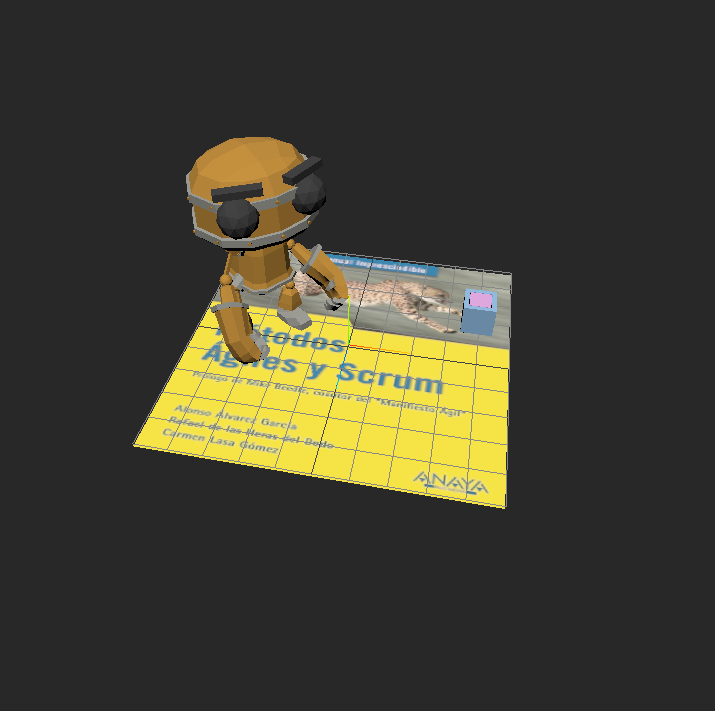
\includegraphics[scale=0.30]{compeditor}
    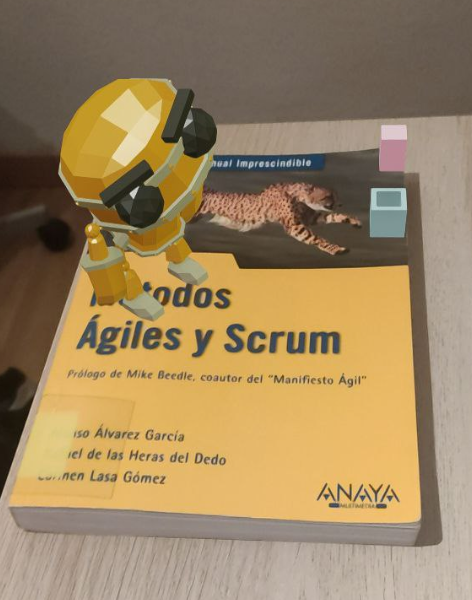
\includegraphics[scale=0.356]{compapp}
    \caption[Comparación de tamaños de modelo en editor y visor]{Comparación de tamaños respecto a la imagen en el editor y en el visor}
    \label{fig:compeditor}
\end{figure}

Este objeto se almacenará en un atributo de clase de la actividad y será el que se ancle a la posición de la imagen desde la función \textit{checkAugmentedImageUpdate}.

\subsection{Escenas por superficie}

Para este tipo de escenas se debe activar el flag de \textit{planeRenderer.isvisible}. Así se visualizará un patrón de puntos en los lugares que identifique la librería como suelos a través de la cámara. También hay que definir el \textit{planeFindingMode}, que determinará las estrategias de búsqueda de superficies que ejecuta \textit{SceneView} como por ejemplo buscar solo superficies horizontales, solo verticales, fijar los puntos de anclaje a la mejor posición estimada, etc. Después de un proceso de prueba se determinó que el que mejores resultados obtenía era \textit{HORIZONTAL}.

%%revisar el planefindingmode

Se definieron dos botones en la interfaz, \textit{Cargar objeto} y \textit{Colocar objeto}. Al iniciarse la actividad únicamente está el primer botón visible. Al pulsarlo, el modelo de la escena aparece en pantalla y comienza a colocarse a la superficie que esté apuntando el usuario. Si el usuario mueve la cámara, el objeto se desplaza acorde. Al pulsar el primer botón este desaparece y aparece el segundo. Cuando se pulsa este el objeto se queda fijo en la posición en la que se encontrara. Llegado a este punto el usuario puede mover el dispositivo como plazca, el objeto seguirá en el mismo punto.

%%cambiar nombre de botones

\subsection{Escenas geoespaciales}

Para emplear escenas geoespaciales era necesario habilitar la API Geoespacial\cite{geospatialapi} de ARCore en la aplicación. Esta es un servicio de \textit{Google Cloud} que provee entre otras cosas de funciones de geoposicionamiento para aplicaciones que usan ARCore. Para ello simplemente se siguieron las instrucciones indicadas en la página para habilitarlo en una sesión de Realidad Aumentada.

Fue necesario habilitar una cuenta de \textit{Google Cloud} para el proyecto. Este es un servicio de pago pero que ofrece una versión gratuita con \$300 de presupuesto, suficientes para el desarrollo. Si se fuera a desplegar la aplicación a nivel comercial sería necesario introducir más presupuesto. El saldo se consume según el número de operaciones que se realicen con la API.

De vuelta al código de la aplicación con todo configurado, solo sería necesario crear un objeto de tipo \textit{Anchor} con las coordenadas GPS almacenadas en \textit{SceneParameters} y asignársela al nodo del modelo creado de forma similar a escenas explicadas anteriormente.

Un problema que surgió fue que el usuario no podía visualizar la escena a menos que estuviera muy cerca de esta. Para solventarlo se aumentó el atributo \textit{sceneView.cameraNode.farClipPlane}, que indica la distancia de renderizado máxima. Hay que tener en cuenta que las aproximaciones GPS en dispositivos móviles siempre son aproximadas hasta cierto punto, así que es posible que si se reproduce la misma escena varias veces el objeto aparezca en lugares ligeramente distintos. 

\subsection{Reproducción de audio y animaciones}

El audio se gestionó con la clase \textit{MediaPlayer}. Esta se encarga tanto de descargar el archivo a través de la \textit{URL} como de reproducirlo al indicárselo. Para las animaciones, la clase \textit{ArModelNode} contaba con soporte para reproducirlas. Solo era necesario indicar el nombre de las animaciones deseadas, los cuales se sacan de \textit{SceneParameters}.

El momento en el que se reproduce el audio y las animaciones dependía del tipo de escena. En imágenes aumentadas comienzan cuando se detecta la imagen activadora en \textit{checkAugmentedImageUpdate}. En el caso de las escenas por superficie es cuando se pulsa el botón de \textit{Colocar objeto}. Con las geospaciales simplemente comienzan cuando la escena se inicia.

\subsection{Menú de selección de escena}

Una vez se inicia sesión se muestra un menú \textit{scrolleable} en el que aparecen todas las escenas creadas por el usuario mostrando su nombre, el tipo de escena y un botón para iniciarla. También hay un botón para cerrar la sesión. Para implementar la lista de escenas se hizo uso de un \textit{RecyclerView}. Este es un tipo de interfaz Android que permite la creación de menús con listas extensas de elementos repetidos. En este caso se repetiría la \textit{``tarjeta''} que representa cada una de las escenas en la interfaz. La peculiaridad que tiene \textit{RecyclerView} con respecto a otras interfaces del estilo, es que solo genera los elementos que se encuentran en un instante determinado en la pantalla del dispositivo. Si el usuario se desplaza por el menú, cargará los elementos nuevos que hayan entrado en pantalla y descartará los anteriores. Con esto se consigue que si un usuario tiene un numero muy grande de escenas, el rendimiento de la aplicación no se vea comprometido.

\section{Backend}

Para el backend se tienen dos elementos. Por un lado, el servicio de \textit{Firebase}, hosteado por Google. Por otro lado, se hizo un servidor web que hace de intermediario entre ambas aplicaciones y \textit{Firebase}. Se van a detallar en los siguientes apartados las configuraciones y desarrollo que se realizó además de justificar las decisiones de diseño.

\subsection{Configuración de la base de datos}

Lo primero fue crear un proyecto en \textit{Firebase}, el \textit{backend-as-a-service} que se utilizaría para la base de datos y autenticación de usuarios. Para ello se siguieron las instrucciones ofrecidas en la propia página. Se generaría una \textit{key} o clave que necesitaría cargarse en cualquier programa que hiciera uso directo de los servicios de \textit{Firebase}. El backend está hosteado \textit{24/7} por Google. Estos servicios tienen opciones de pago profesionales y una gratuita, que para propósitos del desarrollo sería suficiente. Esta simplemente limita la capacidad máxima para almacenar datos en la nube, el número de operaciones de lectura y escritura por día y funcionalidades varias de \textit{Google Cloud}.

Se procedió a configurar la base de datos. \textit{Firebase} utiliza una base de datos no relacional, que a diferencia de las convencionales no emplea tablas que necesiten definirse previamente. En su lugar aquí se tienen \textbf{colecciones}. Estas son conjuntos de \textbf{documentos}, los cuales contienen \textit{campos}. Los documentos tienen en esencia la misma forma que un archivo JSON, y de hecho es el formato que se emplea para el intercambio de información cuando se realizan peticiones a la base de datos. Se creó una colección llamada \textit{escenas} que contendría distintos documentos, cada uno de ellos almacenaría la información sobre una escena, con la misma estructura que se describió en la sección de la aplicación Android. En un inicio se planteó otra colección para almacenar información de los usuarios, pero se descartó en favor del uso de \textit{Authentication}. Los documentos son asignados automáticamente con un código identificador.

\subsection{Usuarios del sistema}

Uno de los servicios que ofrece \textit{Firebase} es \textbf{Authentication}. Este gestiona su propia base de datos de usuario. Para cada usuario almacena un correo electrónico, mantiene todas las contraseñas seguras bajo encriptación y genera automáticamente \textit{ids} de usuario que los identifica inequívocamente. Acciones como registrarse, iniciar sesión, cambiar datos o gestionar los tokens autentificadores se realiza de forma automática y transparente al programador a través de simples llamadas a la librería de \textit{Firebase}. Es por eso que se decidió usar \textit{Authentication} para mantener la información de los usuarios en lugar de crear una colección en la base de datos.

\subsection{Almacenamiento de archivos binarios}

Otro de los servicios de \textit{Firebase} es \textbf{Storage}. Esta interfaz permite almacenar archivos binarios de tamaños elevados. Posteriormente se puede obtener una \textit{URL} a través de la cual descargar el fichero. Estos archivos pueden estar además almacenados en distintas carpetas. Para el proyecto se crearon las carpetas \textit{models}, \textit{audio} e \textit{images}. Cada escena tendría como mínimo un archivo de modelo y como mucho otro de imagen y de audio, así que el nombre de los ficheros almacenados sería la \textit{id} del documento de la escena. Así podrían rescatarse fácilmente al obtener el JSON en la aplicación.

\subsection{Servidor Node.js}

Al igual que con la aplicación web, se usó \textit{Vite} para iniciar un proyecto base de JavaScript con \textit{Node.js}\cite{nodejs} y \textit{Express}\cite{express} para implementar la API que prestaría servicio a las aplicaciones web y de Android. En el archivo \textit{index.js} se definen todas las peticiones que ofrece la interfaz. Cada petición tiene una \textit{URL} asociada. Por ejemplo si se quiere subir una nueva escena, se haría desde la aplicación una petición HTTP POST a la dirección en la que esté alojado el servidor seguido de \textit{/post/escena}. Algunas peticiones tienen implícito en la dirección un parámetro, señalizado con \textit{``:''} en la \textit{URL}. En el caso de \textit{/get/escenas/:idusr}, al hacer la petición se introduce en el \textit{:idusr} el identificador de usuario del que se quieran obtener las escenas. Estas son todas las peticiones que se definieron:

\begin{itemize}
    \item \textit{/get/escenas/:idusr}, para obtener todas las escenas de un usuario concreto.
    \item \textit{/post/escenas}, para subir una nueva escena a la base de datos. Esta se adjunta en el \textit{body} de la petición.
    \item \textit{/update/escenas/:id}, para modificar una escena con un id concreto.
    \item \textit{/delete/escenas/:id}, para borrar una escena.
\end{itemize}

\begin{figure}[h]
    \centering
    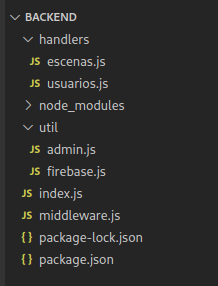
\includegraphics[scale=0.60]{backendfolder}
    \caption[Estructura de archivos de backend]{Estructura de archivos del proyecto de Node.js para el backend}
    \label{fig:backendfolder}
\end{figure}

En la carpeta \textit{util} se almacenan scripts que cargan los objetos \textit{admin} y \textit{db} de \textit{Firebase} a través de los cuales se realizarán las llamadas a la base de datos. En la carpeta \textit{handlers} se encuentran las funciones que gestionan las peticiones de la API. Aquí es donde se hace la conexión con \textit{Firebase} para obtener los datos que se devolverán. Cada función tiene dos argumentos:

\begin{itemize}
    \item \textbf{req}, o request, es el objeto con la información de la petición. Aquí se almacenan los parámetros de la \textit{URL} o el \textit{body}, donde viene incluido archivos adjuntos si fuera el caso.
    \item \textbf{res}, o response, es la respuesta que se envía a la máquina que realizó la petición. Si se realizó una llamada para obtener una lista de escenas, esa información se añadirá en este objeto.
\end{itemize}

\subsection{Esquema y verificación de peticiones}

Se cuenta con tres agentes en la red: \textit{App}, que hace referencia a la aplicación web o Android, el \textit{servidor Node.js} y \textit{Firebase}. Como se ha visto, la aplicación realiza peticiones al servidor Node.js para obtener escenas. Sin embargo, en el caso de identificarse como usuario la aplicación conecta directamente con Firebase en lugar del servidor de Node. Esto podría parecer anómalo pero tiene una razón detrás. Todo el tema de gestión de sesión de usuario viene resuelto ya en las librerías de Firebase para Android y JavaScript. Se tiene un objeto \textit{Authenticator} en memoria, y a través de este se puede crear un nuevo usuario, iniciar sesión, cambiar credenciales, comprobar si la sesión activa es válida, etc. y todo ello de forma segura. Si se quisiera realizar todos esos cálculos desde el servidor Node.js añadiría muchos pasos extra y probablemente quedaría un resultado más pobre, ya que para este proyecto no se cuenta con la experiencia que puede tener un equipo de ingenieros de Google.

Pero, si para el inicio de sesión se prescinde del servidor intermediario, ¿por qué no para todo lo demás? Por dos razones. La primera es que eso supondría programar todas las operaciones de las que se ocupa el servidor en una clase para React y Android Studio, lo cual sería redundante: repetiríamos código en dos proyectos distintos. Si en un futuro se quisiera actualizar alguna de estas funciones, tendría que hacerse por partida doble. Por otro lado teniendo el servidor intermedio obtenemos mayor modularidad. Al final su función es únicamente gestionar las peticiones que se hacen a la base de datos de escenas. Si en un futuro se decidiera sustituir esa base de datos por una opción más conveniente y queriendo mantener el \textit{Authentication} de Firebase para la parte de usuarios, sería posible y fácilmente implementable con la estructura que se propone.

Para asegurar que el usuario que realiza las llamadas es realmente de quien dice ser, se hace uso de \textit{JWT} (\textit{JSON Web Tokens}). Es un estándar con el que se puede propagar entre dos partes y de forma segura la identidad de un usuario. En esencia es una cadena de texto codificada que puede enviarse junto a las peticiones para firmarlas verificando la identidad. El servicio \textit{Authentication} de Firebase genera un \textit{JWT} para cada usuario identificado que se puede obtener desde el cliente. En la implementación llevada a cabo, las aplicaciones envían al servidor por cada petición un token. Este es recibido por el servidor, y antes de atender la petición recibida, comprueba con \textit{Firebase} que el token es válido. Si es el caso, se atiende a la petición y se envía la respuesta. Los tokens tienen validez durante una hora. Una vez transcurrido ese tiempo, \textit{Firebase} genera uno nuevo el cual vuelve a ser obtenible desde la aplicación (figura \ref{fig:esquemabackend}).

\begin{figure}[h]
    \centering
    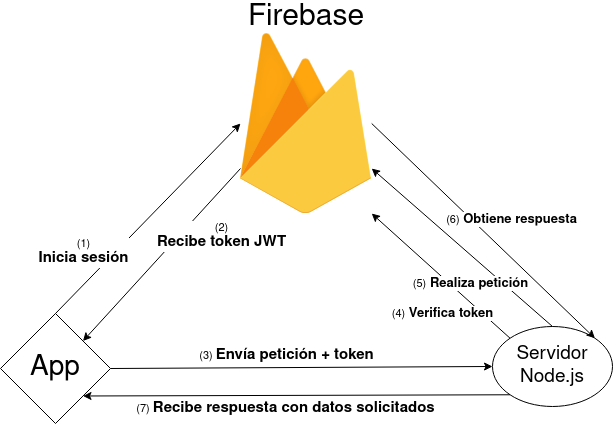
\includegraphics[scale=0.50]{esquema-backend}
    \caption[Diagrama de comunicaciones del servidor]{Diagrama de comunicaciones del servidor}
    \label{fig:esquemabackend}
\end{figure}

En el proyecto de Node.js se realiza esta verificación en la función \textit{decodeToken} dentro del archivo \textit{middleware.js}. Esta comprobación ocurre a cada petición que llega. Si es exitosa comienza a ejecutarse el código que atiende la petición. Si no lo es, devuelve un mensaje de error y termina la comunicación.

\section{Pruebas y corrección de \textit{bugs}}

Para la detección y corrección de \textit{bugs} en el proyecto por un lado se realizaron las pruebas de aceptación definidas en las historias del capítulo 4. Además, se dio la aplicación a probar a varios usuarios, lo cual no solo sirvió para destapar más errores en el sistema, si no para comprobar que la interfaz era intuitiva y manejable.

Cada vez que se descubría algún \textit{bug} en alguna de estas pruebas, se añadía al backlog de la planificación en el sprint correspondiente como una tarea más con la nomenclatura de \textit{FIX-N} y una descripción de el error y por qué fue causado. Los errores encontrados son los siguientes:

\begin{table}[H]
	\resizebox{\textwidth}{!}{%
		\begin{tabular}{|l|l|l|l|l|}
			\hline
			\rowcolor[HTML]{EFEFEF} 
			\textbf{Tarea: FIX-01}           & \textbf{Horas totales: 4}            & \multicolumn{3}{l|}{\cellcolor[HTML]{EFEFEF}\textbf{}} \\ \hline
			\multicolumn{5}{|l|}{\parbox{12cm}{Al cargar el modelo previamente exportado de una escena, el primero de los objetos que la constituyen se mueve de forma independiente, pero el resto de ellos se comportan como si fueran un objeto único, moviéndose a la vez y eliminándose todos si se borra alguno.}}                   \\ \hline
		\end{tabular}%|m{15cm}
	}
\label{FIX-01}
\end{table}

\begin{table}[H]
	\resizebox{\textwidth}{!}{%
		\begin{tabular}{|l|l|l|l|l|}
			\hline
			\rowcolor[HTML]{EFEFEF} 
			\textbf{Tarea: FIX-02}           & \textbf{Horas totales: 1}            & \multicolumn{3}{l|}{\cellcolor[HTML]{EFEFEF}\textbf{}} \\ \hline
			\multicolumn{5}{|l|}{\parbox{12cm}{El usuario crea una escena de tipo marcador. Sube un archivo de imagen y guarda la escena. Vuelve a la lista de escenas. Vuelve a cargar la escena y cambia el tipo a superficie. La imagen desaparece. Guarda la escena, sale del editor y vuelve a entrar. Al cargarse la escena aparece también la imagen aunque ya no sea de tipo marcador.}}                   \\ \hline
		\end{tabular}%|m{15cm}
	}
\label{FIX-02}
\end{table}

\begin{table}[H]
	\resizebox{\textwidth}{!}{%
		\begin{tabular}{|l|l|l|l|l|}
			\hline
			\rowcolor[HTML]{EFEFEF} 
			\textbf{Tarea: FIX-03}           & \textbf{Horas totales: 1}            & \multicolumn{3}{l|}{\cellcolor[HTML]{EFEFEF}\textbf{}} \\ \hline
			\multicolumn{5}{|l|}{\parbox{12cm}{Al borrarse una escena de la base de datos no se eliminan correctamente los archivos asociados como modelos, imágenes y audio.}}                   \\ \hline
		\end{tabular}%|m{15cm}
	}
\label{FIX-03}
\end{table}

\begin{table}[H]
	\resizebox{\textwidth}{!}{%
		\begin{tabular}{|l|l|l|l|l|}
			\hline
			\rowcolor[HTML]{EFEFEF} 
			\textbf{Tarea: FIX-04}           & \textbf{Horas totales: 1}            & \multicolumn{3}{l|}{\cellcolor[HTML]{EFEFEF}\textbf{}} \\ \hline
			\multicolumn{5}{|l|}{\parbox{12cm}{Cuando una sesión dura aproximadamente más de una hora, las conexiones empiezan a fallar con motivo de token inválido. No se soluciona hasta cerrar sesión y volver a iniciarla.}}                   \\ \hline
		\end{tabular}%|m{15cm}
	}
\label{FIX-04}
\end{table}

\begin{table}[H]
	\resizebox{\textwidth}{!}{%
		\begin{tabular}{|l|l|l|l|l|}
			\hline
			\rowcolor[HTML]{EFEFEF} 
			\textbf{Tarea: FIX-05}           & \textbf{Horas totales: 0.5}            & \multicolumn{3}{l|}{\cellcolor[HTML]{EFEFEF}\textbf{}} \\ \hline
			\multicolumn{5}{|l|}{\parbox{12cm}{Cuando se carga un modelo a la escena no se muestra la animación de carga.}}                   \\ \hline
		\end{tabular}%|m{15cm}
	}
\label{FIX-05}
\end{table}

\begin{table}[H]
	\resizebox{\textwidth}{!}{%
		\begin{tabular}{|l|l|l|l|l|}
			\hline
			\rowcolor[HTML]{EFEFEF} 
			\textbf{Tarea: FIX-06}           & \textbf{Horas totales: 0.5}            & \multicolumn{3}{l|}{\cellcolor[HTML]{EFEFEF}\textbf{}} \\ \hline
			\multicolumn{5}{|l|}{\parbox{12cm}{Al introducir manualmente en el navegador la dirección de alguna ruta de enlace protegida, es posible acceder a estas aun sin haber iniciado sesión.}}                   \\ \hline
		\end{tabular}%|m{15cm}
	}
\label{FIX-06}
\end{table}

\begin{table}[H]
	\resizebox{\textwidth}{!}{%
		\begin{tabular}{|l|l|l|l|l|}
			\hline
			\rowcolor[HTML]{EFEFEF} 
			\textbf{Tarea: FIX-07}           & \textbf{Horas totales: 1}            & \multicolumn{3}{l|}{\cellcolor[HTML]{EFEFEF}\textbf{}} \\ \hline
			\multicolumn{5}{|l|}{\parbox{12cm}{Al cargar una escena geoespacial no se cargan en el menú los valores para la posición GPS que hay guardada en el servidor.}}                   \\ \hline
		\end{tabular}%|m{15cm}
	}
\label{FIX-07}
\end{table}

\begin{table}[H]
	\resizebox{\textwidth}{!}{%
		\begin{tabular}{|l|l|l|l|l|}
			\hline
			\rowcolor[HTML]{EFEFEF} 
			\textbf{Tarea: FIX-08}           & \textbf{Horas totales: 0.5}            & \multicolumn{3}{l|}{\cellcolor[HTML]{EFEFEF}\textbf{}} \\ \hline
			\multicolumn{5}{|l|}{\parbox{12cm}{Al reproducir una escena con audio asociado y retroceder al menú de selección de escena la música no se detiene.}}                   \\ \hline
		\end{tabular}%|m{15cm}
	}
\label{FIX-08}
\end{table}

\begin{table}[H]
	\resizebox{\textwidth}{!}{%
		\begin{tabular}{|l|l|l|l|l|}
			\hline
			\rowcolor[HTML]{EFEFEF} 
			\textbf{Tarea: FIX-09}           & \textbf{Horas totales: 0.5}            & \multicolumn{3}{l|}{\cellcolor[HTML]{EFEFEF}\textbf{}} \\ \hline
			\multicolumn{5}{|l|}{\parbox{12cm}{En la aplicación web desplegada no es posible acceder a la página de registro concretamente. Se muestra en pantalla un error 404.}}                   \\ \hline
		\end{tabular}%|m{15cm}
	}
\label{FIX-09}
\end{table}

\section{Despliegue}

En lo que respecta a \textit{Firebase} no hubo que hacer ningún paso adicional para el despliegue a parte de la configuración inicial de cuando se creó el proyecto. El servicio de Google está disponible desde el primer momento. Para que la aplicación Node.js y el editor web pudieran realizar conexiones con el servicio debían cargar en el proyecto un archivo de configuración de \textit{Firebase}. Este es un JSON \textbf{de caracter público}, aunque desde la documentación se recomienda no incluir el contenido del archivo en el código fuente de proyectos de código abierto, ya que, en la mayoría de los casos los usuarios deben crear sus propios proyectos de \textit{Firebase} para dirigir sus apps ahí. Es por ello que se almacena el archivo en el directorio \textit{/ect/secrets} del sistema y se carga desde ahí en el código. Lo mismo ocurre con la clave privada que necesita el proyecto de Node.js para acceder al Admin SDK del servicio.

Para desplegar el servidor web de Node.js y el cliente del editor web se usó \textit{Render}\cite{render}, un servicio en la nube para compilar y ejecutar aplicaciones y webs. Se eligió esta ya que era una de las opciones que se recomendaba en la documentación de \textit{Vite}\cite{vite} además de incluir instrucciones sobre cómo configurarlo. Una de las opciones para cargar las aplicaciones es a través de un repositorio de \textit{GitHub}. Se creó un proyecto de \textit{web service} en \textit{Render} para la aplicación de Node.js y una nueva rama en el repositorio del proyecto llamada \textit{deploy}. Cada vez que hay un nuevo \textit{commit} en esa rama se despliega automaticamente la nueva versión. Se añadió en la configuración del proyecto de \textit{Render} el comando \code{npm install} para obtener todos los paquetes y dependencias del proyecto y  \code{npm start} para ejecutarlo. Además se añadieron ficheros de entorno desde la opción \textit{Environment} para las claves privada y pública de \textit{Firebase} en la dirección mencionada previamente. Después de esperar unos instantes a que realizara el despliegue, se generó una \textit{URL} por la cual acceder al servicio.

Esta \textit{URL} se añadió tanto en el código de la aplicación web como Android en una constante para usarla en las llamadas a la API. No es peligroso exponer la dirección debido a que Node.js solo atiende peticiones con un token de sesión válido.

Para la apliación web se creó un proyecto en \textit{Render} de tipo \textit{static site} y se vinculó con la misma rama del repositorio. Se especificó el comando \code{npm run build} para construir la aplicación con sus dependencias. Se añadió el mismo fichero de entorno que en la aplicación anterior para la clave pública. Siguiendo las direcrices de \textit{Render} para el despliegue de aplicaciones de React que usan React Router, se especificó una regla de reescritura de peticiones para que la librería pudiera gestionar el acceso a las distintas páginas y evitar errores de página no encontrada. Tras esto la aplicación pasaría a construirse y estar disponible a través de una \textit{URL} (figura \ref{fig:render}).

\begin{figure}[h]
    \centering
    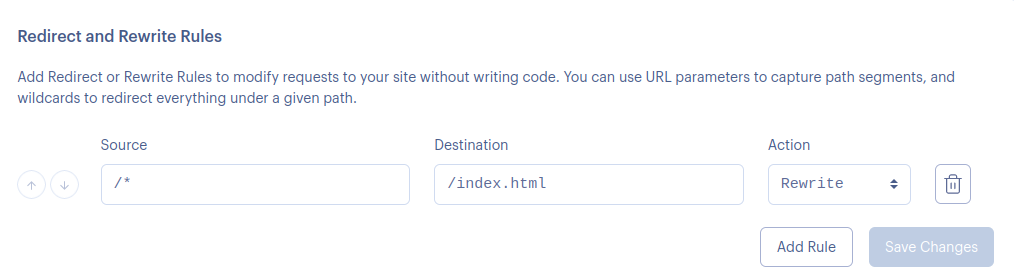
\includegraphics[scale=0.4]{render}
    \caption[Reescritura de peticiones para React Router]{Configuración de reescritura para React Router en el despliegue de la aplicación web.}
    \label{fig:render}
\end{figure}

Para la aplicación Android se generó una \textit{APK} (archivo instalador) desde el propio IDE en el menú de \textit{Build}, \textit{Build Bundle(s)/APK(s)}, \textit{Build APK(s)}.

	% Presupuesto

	% Conclusiones
	\chapter{Conclusiones y trabajos futuros}

En este capítulo se verán las conclusiones del trabajo realizado, el cumplimiento de los objetivos establecidos en el capítulo 2 y 4 los el trabajo futuro que se podría realizar sobre el proyecto.

\section{Conclusiones}

Respecto a los objetivos del proyecto definidos en el capítulo 2 se tiene que:

\begin{itemize}
    \item \textbf{OBJ-1}: Se propuso hacer una herramienta para la composición de escenas 3D a través de modelos importados o creados. Se ha logrado desarrollar una aplicación web que permite la carga de archivos y la manipulación de los mismos con las transformaciones de translación, rotación y escalado. Si bien a partir de estos modelos se pueden realizar composiciones y fusionarlos todos en un único fichero, hay que matizar que por falta de tiempo el software no puede generar las geometrías básicas con las que hubiera sido posible construir objetos 3D sencillos. Esto último habría sido un buen añadido pero en ningún momento obstaculiza el propósito del sistema. Los usuarios siguen siendo capaces de construir escenas con gran libertad a partir de modelos que pueden encontrar en internet.
    \item \textbf{OBJ-2}: Se pretendía que el software fuera sencillo, intuitivo y que no requiriera experiencia previa en la manipulación de entornos 3D. Esto se ha logrado con una interfaz limpia y minimalista que da las opciones esenciales sin abrumar al usuario. El uso de gizmos hace que sea fácil interactuar con los elementos de la escena y en ningún momento se utilizan tecnicismos como \textit{keyframes} que una persona puede no entender.
    \item \textbf{OBJ-3}: La reproducción de animaciones y audio de escena otorgan de dinamismo y frescura a las composiciones. Aun disponiendo únicamente de las tres herramientas básicas para la manipulación de modelos, el usuario puede crear escenas vistosas sin haber comprometido la complejidad de la interfaz.
    \item \textbf{OBJ-4}: Se quería desarrollar un software para la visualización de experiencias de realidad aumentada compuestas de modelos 3D. Esto se ha logrado gracias a la aplicación Android, que es capaz de reproducir escenas tanto de posición en superficies, imágenes aumentadas e incluso geoespaciales con coordenadas GPS. El resultado es vistoso y la aplicación es fácil de navegar.
    \item \textbf{OBJ-5}: Se requería que el sistema pudiera almacenar las escenas creadas por el usuario para poder recuperarlas y editarlas desde el propio sistema. Esto se realizó gracias a un servidor web con base de datos y gestión de cuentas de usuario de forma segura. Los usuarios inician sesión tanto en el editor web para crear y almacenar sus composiciones como en la aplicación Android para reproducir las mismas.
\end{itemize}

Este proyecto consigue aportar a otras propuestas similares una opción más sencilla en el buen sentido de la palabra además de tener la opción de reproducción nativa en dispositivo móvil y la creación de escenas geoespaciales con coordenadas GPS. Aunque el resultado final es un sistema cerrado (en el sentido de que consta de distintas partes conectadas e interdependientes), sus distintos elementos tienen valor por separado. No sería descabellado pensar que el código del editor o de la aplicación Android fueran de utilidad para usarlos de base a la hora de crear otros proyectos relacionados o integrándolos en aplicaciones mayores. En lo personal este trabajo ha supuesto un gran reto ya que hasta el momento no había construido una aplicación completa de principio a fin hasta ser desplegada. Se ha obtenido una visión mucho más amplia sobre cómo encarar proyectos de este estilo. Y aunque hayan surgido problemas y contratiempos, se considera que se han resuelto de una forma más que competente con el conocimiento y los recursos de los que se disponían.

\section{Trabajos futuros}

Para trabajos futuros sobre el proyecto se proponen los siguientes puntos, en los que se tienen tanto ideas adicionales que no se propusieron hasta ahora como deudas pendientes que no dio tiempo a desarrollar:

\begin{itemize}
    \item La historia de usuario RA-12.1 quedó pendiente de implementarse. Trata de añadir ciertos criterios de filtro a la lista de escenas como por nombre o por tipo para poder localizarlas más rapidamente. Esto es especialmente importante para los usuarios que hagan un uso algo más intensivo de la aplicación y acaben con un listado extenso.
    \item Las historias de usuario RA-09 y RA-09.1 permitirían al usuario la creación de geometrías básicas que usar como bloques de construcción para composiciones sencillas, haciendo que este no dependa tanto de los recursos que sea capaz de encontrar en internet.
    \item La historia de usuario RA-03. Sería interesante que se tuviera la opción de en una misma escena definir distintas imágenes activadoras y que se visualizara un modelo u otro dependiendo del marcador enfocado.
    \item Tener reproducción nativa de escenas es una baza, pero es a costa de solo haber podido desarrollar una aplicación Android. En un futuro se podría implementar una app similar para \textit{iOS} y así tener cubierto a todo el mercado de dispositivos móviles.
    \item Se podría implementar una herramienta para anidar modelos en el editor. De la misma manera que \textit{Three.js} representa una escena con nodos en un grafo de árbol, el usuario podría definir que un modelo sea el padre de uno u varios modelos más para que estos lo sigan en cualquier transformación que se le aplique sin necesidad de estar seleccionándolos cada vez.
\end{itemize}

\section{Errores conocidos}

Se enumeran aquí los errores conocidos del proyecto pero que por tiempo o recursos no han podido solucionarse:

\begin{itemize}
    \item En el aviso para dispositivos incompatibles de la aplicación web se mostraba una imagen de un portátil. Esta imagen da error al ser cargada en la versión desplegada.
    \item En ocasiones muy puntuales, al abrir la aplicación web en un navegador con sesión previamente iniciada, las lista de escenas tarda mucho en aparecer.
    \item Con ciertas cámaras e iluminaciones, en el modo de imágenes aumentadas de la aplicación Android pueden percibirse movimientos repentinos del modelo intentando colocarse sobre la imagen.
\end{itemize}

	% Trabajos futuros


	
	\newpage
	\bibliography{bibliografia}
	\bibliographystyle{plain}
	
\end{document}

